\chapter{Analyse des Lastenhefts}
Legende:

\question{Fragen sind in rot verfasst.}

\answer{Die dazugehörigen Antworten sind darunter in blau erläutert.}

\section{Einleitung}
Für unser sehr erfolgreiches Startup-Unternehmen im Bereich Event-Management benötigen wir ein neues Planungssystem, um alle Event-Daten noch besser und effizienter erfassen und verwalten zu können.

\question{Wo befindet sich das Unternehmen? In welcher Rechtslage befindet sich das Unternehmen?}

\answer{Das Unternehmen hat seinen Hauptsitz in Deutschland.}

\question{Wo werden die Daten gespeichert? Intern oder Extern? Wenn intern, welche Infrastruktur ist vorhanden? Wenn extern, wie wichtig ist der Datenschutz?}

\answer{Die Daten werden auf unseren internen Ressourcen gespeichert. Diese Infrastruktur ist derzeit schon verfügbar.}

\question{Wie viele Mitarbeiter hat das Startup-Unternehmen?}

\answer{Wir beschäftigen derzeit 69 Mitarbeiter und stellen fortlaufend neue ein.}

Dabei planen und veranstalten wir Events mit Teilnehmerzahlen bis ca. 1000 Personen (Kongresse, Hochzeiten, Empfänge, Vernissagen, Sportveranstaltungen, Wettbewerbe, Konzerte usw.). Die meisten Events führen wir für 50 - 100 Teilnehmer durch.

\question{Gibt es eine Mindestanzahl an Teilnehmern? Kann es auch keine Teilnehmer zu einem Event geben?}

\answer{Nein, es kann nicht vorkommen, dass es zu einem Event keine Teilnehmer gibt. Es gibt allerdings auch keine Mindestanzahl an Teilnehmern. Die erwähnten 50-100 Teilnehmer sind lediglich ein Richtwert.}

\question{Müssen die einzelnen Teilnehmer erfasst werden oder ist nur die Teilnehmeranzahl wichtig? Welche Attribute sind für Teilnehmer notwendig?}

\answer{Die Teilnehmeranzahl muss nicht festgehalten werden.}

\newpage

\question{Sollen Einladungen an Teilnehmer versendet werden können?}

\answer{Die Planungssoftware ist nur für das Planen und Organisieren von Events vorgesehen. Die Verwaltung der Teilnehmer ist darin nicht vorgesehen. }

\question{Müssen Zusagen und Absagen von Teilnehmern erfasst werden?}

\answer{Wie zuvor erwähnt, dient die Software nicht der Verwaltung und Überprüfung der Teilnehmer, weshalb auch keine Zusagen beziehungsweise Absagen erfasst werden müssen. Diese Daten erhalten wir von unseren Partnern, die das Ticketing übernehmen. }

\question{Müssen Umfragen an Teilnehmer (Bsp: Essensauswahl) versendet werden können? Sollen die Antworten im System erfasst werden?}

\answer{Nein, auch diese Fragen werden durch unsere Ticketing-Partner entgegengenommen und unseren Mitarbeitern übermittelt. Diese tragen anschließend die kalkulierten Daten zur Planung ein.}

\question{Ist eine Gruppierung von Teilnehmern notwendig? Beispiel: Geimpfte und nicht geimpfte Teilnehmer? Gruppierung nach Volljährigkeit erforderlich?}

\answer{Nein, das ist nicht notwendig. Unsere Ticketing-Partner übernehmen das.}

\question{Sollen die Eventkategorien verschieden betrachtet werden? Gibt es verschiedene Funktionalitäten für verschiedene Eventkategorien?}

\answer{Nein, alle Eventkategorien können gleich betrachtet werden. Es sollen keine verschiedenen Funktionalitäten vorhanden sein. Es gibt jedoch unterschiedliche Event-Elemente, welche eine Templatefunktionalität für verschiedene Eventkategorien darstellen.}

\question{Sind die Eventkategorien vordefiniert oder sollen diese erweitert werden können?}

\answer{Die Kategorie soll frei wählbar sein.}

\question{Müssen im System externe Firmen beachtet werden? Werden externe Mitarbeiter für kurze Zeit eingestellt? Gibt es Praktikanten?}

\answer{Es werden die Kontaktdaten zu externen Firmen benötigt. Es sollen jedoch keine technischen Schnittstellen angeboten werden. Alle Mitarbeiter werden gleich behandelt. Um den Praktikanten ein nahes Verständnis und optimale Erfahrungen bei uns zu ermöglichen werden sie wie Mitarbeiter behandelt. Es können auch externe Helfer in einer Gruppe unterstützend mitwirken, diese werden jedoch nicht als Mitarbeiter im System gepflegt.}

\question{Müssen Rechnungen gedruckt werden?}

\answer{Nein, das übernimmt das vorhandene Finanzsystem.}

\newpage

\question{Gibt es Events, die nur geplant und von einem anderen Unternehmen  durchgeführt werden?}

\answer{Nein, alle Events werden von uns geplant und durchgeführt.}


Bisher vor kurzem war es möglich, mit Hilfe von Excel die Planung und Verwaltung unserer Events durchzuführen, was durch die stark steigende Anzahl an Events nun nicht mehr auf Dauer realisierbar ist.

\question{Was passiert mit den bereits vorhandenen Daten aus den Excel Dateien? Wie werden diese in das neue System übertragen?}

\answer{Die Daten werden von Hand von einem unserer Mitarbeiter übertragen.}

\question{Was bedeutet stark steigende Anzahl an Events? Wie viele Events sind dabei gemeint?}

\answer{Früher führten wir wöchentlich ein bis zwei Events durch. Heute führen wir bis zu zehn Events in der Woche durch.}

\section{Lastenheft}
\subsection{Zielsetzung}
Ziel des Entwicklungsauftrags ist eine Software für die Planung und Durchführung von Veranstaltungs-Events. Alle Daten sollen zentral gespeichert werden, da mehrere Benutzer gleichzeitig auf die Daten und Termine zugreifen werden.

\question{Wie viele Benutzer nutzen die Software gleichzeitig?}

\answer{Etwa 20 bis 30 Mitarbeiter sollen die Software gleichzeitig nutzen können.}

\question{Was ist mit zentral genau gemeint?}

\answer{Die Daten sollen sich in einem Verzeichnis auf einem Server befinden.}

\question{Wie genau müssen die Termine sein? Auf Wochen, Tage, Stunden oder Minuten genau?}

\answer{Die Termine sollen auf Minuten genau festgelegt werden können.}

\question{Welches Datumsformat soll verwendet werden?}

\answer{Nach dem Format TT.MM.JJJJ HH:MM. Die Zeit ist dabei im 24-Stunden-Format anzugeben. Beispiel: 01.04.2021 14:35}

Ein selektiver Import und Export von Daten über lesbare Dateien muss für Backups und zum Datenaustausch möglich sein.

\newpage

\question{Muss das importiert werden können, was exportiert werden kann?}

\answer{Ja, da die Exporte auch für die Backups verwendet werden.}

\question{Welche Importformate sind relevant?}

\answer{Es soll eine CSV Datei importiert werden können.}

\question{Welche Exportformate sind relevant?}

\answer{Es soll eine CSV Datei exportiert werden können.}

\question{Ist auch ein Export zu einem Drucker gewünscht?}

\answer{Nein, wir sind ein umweltorientiertes und modernes Unternehmen. Daher möchten wir Ausdrucke auf Papier vermeiden.}

\question{Welche Daten sollen exportiert und importiert werden können? Soll nur ein Teil der Daten exportiert werden können? Soll nur ein Teil der Daten importiert werden können?}

\answer{Es sollen selektiv ganze Events exportiert werden können. Dazu gehören alle Teilevents, die Hilfsmittel und die zugeordneten Mitarbeiter. Wir wollen ebenfalls ganze Events importieren. Dabei kann ausgewählt werden, welche Events aus einer Datei importiert werden sollen.}

\question{Was bedeutet selektiv? Nach welchen Kriterien soll selektiert werden können? Was soll selektiert werden können?}

\answer{Events sollen direkt oder über Filter ausgewählt werden können. Es soll nach allen Attributen des Events gefiltert werden können.}

\question{Wie fein kann die Selektion werden? Kann von einem Event nur ein Teil exportiert oder importiert werden? Zum Beispiel nur die Materialien zum Event?}

\answer{Für uns reicht es aus ein ganzes Event exportieren und importieren zu können.}

\question{Wie soll selektiert werden, was importiert wird?}

\answer{Nachdem eine Datei für den Import ausgewählt wurde, soll eine intuitive Benutzeroberfläche angezeigt werden. Es soll eine Auswahlliste angezeigt werden, um Events direkt auszuwählen. Zudem sollen Filter auf die Liste der importierbaren Events angewendet werden können.}

\question{Wie soll selektiert werden, was exportiert wird?}

\answer{In einer Übersicht von Events soll es möglich sein, die Events zu filtern und über Checkboxen Events zu selektieren. Dabei soll es auch möglich sein, alle angezeigten Events auf einmal zu selektieren.}

\newpage

\question{Was ist mit Datenaustausch gemeint? Ist damit der Austausch mit anderer Software gemeint?}

\answer{Damit ist gemeint, dass mit Menschen die Daten ausgetauscht werden können. Ein Import ist nur in das zu entwickelnde System notwendig.}

\question{Ist ein Import und Export über Schnittstellen notwendig? Wie sollen diese Schnittstellen aussehen? Wird nur ein Import über Dateien erwartet?}

\answer{Wir brauchen nur einen Import über Dateien. Weitere Schnittstellen sehen wir nicht als notwendig an.}

\question{Wer darf exportieren und importieren?}

\answer{Alle Organisatoren und der Administrator dürfen exportieren und importieren.}

\question{Soll ein Import und Export geloggt werden?}

\answer{Der Import und Export soll geloggt werden. Dabei sind der Zeitpunkt, der Eventname und der Nutzer wichtig.}

\question{Was soll passieren, wenn Daten importiert werden, die bereits vorhandenen Daten widersprechen?}

\answer{Es soll eine Meldung erscheinen und der Nutzer kann dann entscheiden, ob die Daten überschrieben werden oder das entsprechende Event übersprungen wird.}

\question{Was soll passieren, wenn Daten importiert werden, die bereits vorhanden sind?}

\answer{Es soll eine Meldung erscheinen und das entsprechende Event wird übersprungen.}

\question{Was soll passieren, wenn Importdaten invalide sind?}

\answer{Es soll eine Meldung erscheinen und der Nutzer kann dann entscheiden, ob das entsprechende Event übersprungen wird oder er den kompletten Import abbrechen möchte.}

\question{Kann ein Import rückgängig gemacht werden?}

\answer{Nein, das ist für uns nicht notwendig.}

\question{Wie oft werden Backups durchgeführt?}

\answer{Wir wollen wöchentlich ein komplettes Backup.}

\question{Wo werden die Backups gespeichert?}

\answer{Die Backups werden auf Magnetbändern gesichert. Die Magnetbänder werden in einem anderen Gebäude gelagert.}

\newpage

\question{Werden die Backups automatisch oder manuell ausgeführt? Werden die Backups automatisch ausgeführt, welche Konfigurationsmöglichkeiten gibt es? Wer darf diese Konfiguration vornehmen?}

\answer{Die Backups sollen automatisch ausgeführt werden. Dabei kann ein Administrator den Zeitpunkt des wöchentlichen Backups einstellen oder ein manuelles Backup durchführen. Das Zielverzeichnis des Backups muss einstellbar sein.}

\question{Wie lange werden Backups aufbewahrt?}

\answer{Ein Backup soll 20 Jahre aufbewahrt werden.}

\question{Muss das Backup verschlüsselt werden?}

\answer{Nein, das brauchen wir nicht. Die Magnetbänder sind pyhsisch ausreichend abgesichert.}

\question{In welchem Format sollen die Backups erstellt werden?}

\answer{Damit die Backups importiert werden können, soll das gleiche Format wie bei einem Export verwendet werden.}

\question{Sollen Backups inkrementell oder immer vollständig durchgeführt werden?}

\answer{Backups sollen immer vollständig durchgeführt werden.}

Eine intuitive, leicht bedienbare Benutzeroberfläche setzen wir als selbstverständlich voraus. Es sollen keine besonderen Computerkenntnisse zur Bedienung der Software erforderlich sein. 

\question{Auf welchen Endgeräten soll die Software verwendet werden? Ist eine Touchbedienung vorgesehen?}

\answer{Die Software soll vorerst auf Laptops verwendet werden. In Zukunft ist vorgesehen, die Verwendung von anderen Endgeräten zu evaluieren und unter Umständen auf Tablets umzusteigen. Da unsere Laptops mit Touch-Funktionalität ausgestattet sind, ist auch eine Bedienung darüber zu beachten. Auch eine Verwendung über Maus und Tastatur soll unterstützt werden, da einige Mitarbeiter diese bevorzugen.}

\question{Muss Barrierefreiheit beachtet werden?}

\answer{Es müssen keine besonderen Vorkehrungen für die Barrierefreiheit getroffen werden.}

\question{Soll die Software über die Tastatur bedienbar sein?}

\answer{Ja, da Mitarbeiter täglich mit dem Programm arbeiten, soll es möglich sein für erhöhte Produktivität möglichst alle Tätigkeiten mit Tastatureingaben zu bedienen.}

\question{Wie groß sind die Bildschirme der Endgeräte? }

\answer{Die verwendeten Laptops haben eine Bildschirmdiagonale von 15 Zoll.}

\question{Sollen Schulungen zur Software angeboten werden?}

\answer{Wir wollen unsere Mitarbeiter nicht mit Schulungen über ihre normalen Tätigkeiten hinaus weiter belasten. Daher möchten wir eine möglichst intuitive Software, die von Nutzern mit Erfahrung in gängigen Programmen leicht bedient werden kann.}

\question{In welchen Sprachen soll die Benutzeroberfläche verfügbar sein?}

\answer{Da wir ein rein deutsches Unternehmen sind und nicht planen unsere Tätigkeiten in naher Zukunft auf das Ausland zu erweitern oder internationale Mitarbeiter einzustellen, muss die Software nur in deutscher Sprache verfügbar sein.}

\question{Soll es für unterschiedliche Rollen unterschiedliche Oberflächen geben?}

\answer{Für die verschiedenen Rollen sollen im gleichen Programm bestimmte Anzeigen ausgeblendet werden.}

\question{Soll die Benutzeroberfläche personalisierbar sein?}

\answer{Nein, die Benutzeroberfläche soll unternehmensweit einheitlich gehalten werden, damit Mitarbeiter sich einfach untereinander in der Bedienung helfen und gegenseitig anlernen können.}

\subsection{Anwendungsbereiche}
Die Software soll ausschließlich für die Planung und Verwaltung von Events, Kunden, Ausrüstung, Locations und Angestellten und den damit direkt verbundenen Elementen verwendet werden. Sie soll im Alltag auf Laptops eingesetzt werden.

\question{Haben die Laptops eine dauerhafte Internetverbindung? Soll die Anwendung auch offline funktionieren?}

\answer{Es kann davon ausgegangen werden, dass die Laptops immer Zugriff auf das zentrale Datenverzeichnis haben. Es kann nicht davon ausgegangen werden, dass die Laptops immer eine Verbindung mit dem World Wide Web haben.}

\question{Welche Leistung haben die Laptops?}

\answer{Die Laptops sind in der Leistung handelsüblich und wurden 2019 angeschafft.}

\question{Welche Betriebssysteme werden auf den Laptops eingesetzt?}

\answer{Einige Laptops laufen unter Windows 10, andere jedoch auch unter macOS. Keine weiteren Betriebssysteme werden verwendet oder müssen hier berücksichtigt werden.}

\question{Wird die Software unter außergewöhnlichen Umständen nicht auf einem Laptop verwendet?}

\answer{Die Software wird nach heutigem Stand immer auf Laptops verwendet.}

\subsection{Zielgruppen, Benutzerrollen und Verantwortlichkeiten}
Es soll verschiedene Benutzerrollen geben:

\begin{itemize}
    \item Organisatorinnen und Organisatoren pflegen die jeweiligen Event-Daten
    
    \question{Was sind Event-Daten? Sind damit alle Daten eines Events gemeint?}

    \answer{Event-Daten sind alle Daten, die dem Event zugehörig sind. Also alle Attribute und alle Daten der zugehörigen Teilevents.}

    \question{Können Organisatoren neue Events anlegen? Können Organisatoren Events löschen?}

    \answer{Ja, Organisatoren können neue Events anlegen. Ja, Organisatoren können Events auch löschen. Wenn ein Event gelöscht wurde, soll es innerhalb von 14 Tagen wiederhergestellt werden können.}

    \question{Können Organisatoren die Events anderer Organisatoren verändern?}

    \answer{Nein, ein Event kann immer nur von dem dazugehörigen Organisator bearbeitet werden.}

    \question{Können Organisatoren alle Events sehen? Wenn nein, können Organisatoren Events mit anderen Organisatoren teilen?}

    \answer{Um eine gute Kollaboration und einen Austausch zwischen erfahrenen und neuen Organisatoren zu ermöglichen, können Organisatoren alle Events standardmäßig einsehen. Es werden auch keine vertraulichen Events geplant, die Vorkehrungen bei der Sicherheit der Daten benötigen würden.}

    \item Beschaffungspersonal (besorgen und verwalten benötigte Utensilien, die mehrfach verwendet werden können). Es hat lesenden Zugriff auf von Organisatorinnen und Organisatoren freigegebene Teilevents. Sie können in Gruppen organisiert sein (d.h. es gibt eine/n Gruppenleiterin bzw. einen Gruppenleiter) für Aktionen, die nicht oder nur schwer allein zu realisieren sind. 
    
    \question{Kann jeder Mitarbeiter Teil einer Gruppe sein?}

    \answer{Ja, jeder Mitarbeiter kann Teil einer Gruppe sein.}
    
    \question{Sieht das Beschaffungspersonal auch das Event zu einem zugehörigen Teilevent?}

    \answer{Das Beschaffungspersonal sieht bloß das zugewiesene Teilevent und um dieses im korrekten Kontext platzieren zu können, sind auch die Eltern-Teilevents bis zum Event selbst sichtbar, nicht jedoch Geschwister-Teilevents. Bei fehlenden Informationen im Teilevent soll dem Beschaffungspersonal die Möglichkeit gegeben werden, den Organisator zu kontaktieren.}

    \question{Was genau ist eine Gruppe? Ist es ähnlich einer Abteilung im Unternehmen oder eher eine lose Sammlung an Menschen, die gemeinsam nur für diese Aufgabe versammelt werden?}

    \answer{Eine Gruppe ist eine Menge an Menschen, die einem bestimmten Teilevent zugewiesen sind. Wir sind ein modernes und flexibles Unternehmen, welches sich nicht unnötig durch strikte Organisationsstrukturen einschränken möchte, daher haben wir keine festen Teams.}

    \question{Kann eine Gruppe an mehreren Teilevents arbeiten?}

    \answer{Nein, eine Gruppe ist kein übergeordnetes Konzept, wie eine Abteilung. Eine Gruppe existiert immer nur für das bestimmte Teilevent.}

    \question{Wer kann Teilnehmer zu einer Gruppe hinzufügen oder entfernen?}

    \answer{Der Organisator verwaltet die bearbeitende Gruppe an Benutzern. Er weist dieser Personen zu und kann sie auch wieder entfernen. Der Organisator wählt beim Erstellen der Gruppe eine Person als Gruppenleiter aus und kann auch nachträglich den Gruppenleiter bestimmen. Eine Gruppe hat immer genau einen Gruppenleiter.}

    \question{Wenn ein Teilevent keine Gruppe hat, wird das Teilevent dann von einem einzelnen Benutzer bearbeitet oder ist der Nutzer in einer eigenen Gruppe als Gruppenleiter?}

    \answer{Wenn ein Teilevent von einer Einzelperson bearbeitet wird, ist diese nicht Teil einer Gruppe nur mit sich selbst. Es können nur Gruppen mit mindestens zwei Personen existieren.}

    \question{Kann eine Gruppe an mehreren Teilevents gleichzeitig arbeiten?}

    \answer{Nein, eine Gruppe ist, wie bereits beschrieben, nur als Sammlung von Personen für dieses bestimmte Teilevent vorhanden. Mitarbeiter können aber an mehreren Teilevents gleichzeitig arbeiten und dabei auch in verschiedenen Gruppen gleichzeitig sein. Dadurch möchten wir es ermöglichen, dass erfahrene Mitarbeiter eigenständig planen, wie sie ihre Zeit zwischen mehreren simultanen Tätigkeiten einteilen.}

    \question{Sind Aktionen Teilevents?}

    \answer{Ein Teilevent ohne untergeordnete Teilevents beschreibt immer genau eine durchzuführende Aktion. Eine Aktion ist somit ein Teilevent, welchem keine Unter-Teilevents zugeordnet sind und Hilfsmittel zugeordnet werden können.}
    
    \item Personalmitarbeiter pflegen Mitarbeiterdaten im System 
    
    \question{Was sind Mitarbeiterdaten? Welche Daten zu einem Mitarbeiter werden gepflegt?}
    \answer{Zu einem Mitarbeiter gehören:}
    \begin{itemize}
        \item \answer{Name}
        \item \answer{Personalnummer (fortlaufende Nummer)}
        \item \answer{Anschrift}
        \item \answer{Telefonnummer}
        \item \answer{Mail-Adresse}
        \item \answer{Rollen}
        \item \answer{Beschäftigungszeiträume (Start- und Enddatum. Das Enddatum ist optional)}
    \end{itemize}

    \question{Wie pflegen Personalmitarbeiter Mitarbeiterdaten?}

    \answer{Mitarbeiterdaten sollen über eine intuitive Benutzeroberfläche im Programm gepflegt werden.}

    \question{Können Personalmitarbeiter anderen Nutzern Rollen zuweisen? Beispiel: Personalmitarbeiter weißt einem Nutzer die Rolle Organisator zu. Wenn ja, welche Rollen kann ein Personalmitarbeiter anderen zuweisen?}

    \answer{Ja, Personalmitarbeiter weisen den Nutzern ihre Rollen zu. Ein Personalmitarbeiter kann jede Rolle zuweisen.}

    \question{Haben Personalmitarbeiter ihnen zugewiesene Mitarbeiter oder pflegen sie die Daten aller Mitarbeiter?}

    \answer{Personalmitarbeiter sind für die Pflege aller Mitarbeiter zuständig. Wir sind bisher ein kleines Unternehmen, welches nur wenig Personalmitarbeiter benötigt. Jedoch möchten wir, dass jede Aktion des Personalmitarbeiters mit Datum und Namen des Verantwortlichen festgehalten wird.}

    
    \item Montageleiterinnen und Montageleiter (Leitung von Mitarbeitern für den Auf- und Abbau der benötigten Geräte, Bauten und Einrichtungen). Die Rolle soll lesenden Zugriff auf alle Daten haben, die in ihren Arbeitsbereich fallen.
    
    \question{Sind Montageleiter Gruppenleiter? (Siehe Beschaffungspersonal) }

    \answer{Montageleiter können Gruppenleiter sein. Montageleiter ist eine bestimmte Rolle im System und Gruppenleiter ist der Hauptverantwortliche einer Gruppe.}

    \question{Wer teilt dem Montageleiter seinen Arbeitsbereich zu?}

    \answer{Der Organisator des entsprechenden Events teilt dem Montageleiter seinen Arbeitsbereich für das Event zu.}

    \question{Welche Daten gehören zu einem Arbeitsbereich?}

    \answer{Einem Montageleiter ist jeweils ein Teilevent zugewiesen, welches damit sein Arbeitsbereich ist. Damit kann dieser dann auf das Teilevent und auf übergeordnete Teilevents zugreifen. Des Weiteren können Monatageleiter auch auf alle Elemente zugreifen, die einem für ihn sichtbaren Teilevent zugewiesen sind. Das wären zum Beispiel Hilfsmittel und Bilder.}

    \question{Sind Montageleiter einem bestimmten Teilevent oder Event zugewiesen?}

    \answer{Einem Teilevent, welches der Montage dienen soll, ist immer ein Montageleiter zugewiesen.}

    \question{Haben die Mitarbeiter, welche von den Montageleitern angeleitet werden, Zugriff auf das System? Falls ja, welche Rolle haben diese?}

    \answer{Ein Helfer kann entweder einer unserer Mitarbeiter oder eine externer Helfer sein. Unsere Mitarbeiter haben ihre normale Rolle und benötigen keine weitere, um als Helfer bei einer Montagetätigkeit mitzuwirken. Externe Helfer haben keinerlei Zugriff auf das System.}

    \question{Sind die Mitarbeiter, welche von den Montageleitern angeleitet werden, im System hinterlegt?}

    \answer{Externe Helfer, wie zum Beispiel die Oma, die noch bei der Deko helfen will, sollen in einer Gruppe mit Namen hinterlegt werden. Dadurch können wir sie als Helfer für diese Tätigkeit festhalten und nicht weiter verwalten.}

    \question{Haben Montageleiter ein festes Team mit dem sie arbeiten?}

    \answer{Nein, Montageleiter haben kein festes Team.}
    
    \item Eine hauptverantwortliche Person (Administrator) hat Vollzugriff auf sämtliche Daten, vor allem für deren Import und Export sowie deren Backup. 
    
    \question{Gibt es etwas, was der Administrator nicht darf?}

    \answer{Der Administrator darf alles machen, was irgendein Nutzer tun könnte.}

    \question{Kann es mehrere Administratoren geben?}

    \answer{Ja, es kann mehrere Administratoren geben}

    \question{Wer kann einem Nutzer die Administratorrolle zuweisen?}

    \answer{Das System startet mit einem Administratorkonto und weitere Mitarbeiter können von Personalmitarbeitern oder Administratoren die Rolle Administrator zugewiesen bekommen.}

    \question{Kann nur der Administrator einen Import, einen Export und Backups auslösen?}

    \answer{Nein, auch Organisatoren können diese Funktionen nutzen. Jedoch kann nur der Administrator ein Backup erstellen.}

\end{itemize}

\newpage

\question{Sollen weitere Benutzerrollen hinzugefügt werden können? Sollen die Berechtigungen der Rollen veränderbar sein?}

\answer{Aus Sicherheitsgründen möchten wir die vorhandenen Rollen nicht verändern oder neue hinzufügen.}

\question{Wie viele Benutzerrollen kann ein Benutzer haben?}

\answer{Ein Benutzer kann alle Rollen gleichzeitig haben.}

\question{Werden die Benutzerrollen über die Software oder über ein anderes Programm verwaltet?}

\answer{Die Benutzerrollen werden über das System von Personalmitarbeitern zugewiesen.}

\question{Wie wird einem Nutzer eine Rolle zugewiesen?}

\answer{Ein Nutzer erhält seine Rolle entweder von einem Personalmitarbeiter oder dem Administrator. Das Administratorkonto ist zu Beginn bereits vorhanden.}

\question{Wie können die Nutzer verwaltet werden?}

\answer{Nutzer werden von den Personalmitarbeitern erstellt, gelöscht oder geändert.}

\question{Gibt es ein externes Authentifizierungssystem, das verwendet werden kann? Ist ein Single-Sign-On gewünscht?}

\answer{Es gibt kein unternehmensweites Authentifizierungssystem, das hier berücksichtigt werden könnte.}

\question{Wenn ein Benutzer Rechte hat, die Daten eines Teilevent einzusehen, hat der Benutzer dann auch die Rechte die übergeordneten Events zu sehen?}

\answer{Ja, damit unsere Mitarbeiter immer den nötigen Kontext für die Erledigung ihrer Aufgaben haben, sehen diese auch die übergeordneten Events und Teilevents des ihnen zugewiesenen Teilevents.}

\subsection{Zusammenspiel mit anderen Systemen}
Die Daten über die Angestellten (Gehälter bzw. Löhne, Steuern, Kranken- und Rentenversicherung usw.) werden separat durch ein vorhandenes Personalbuchhaltungsprogramm verwaltet und müssen hier nicht berücksichtigt werden. Die finanztechnischen Daten werden über unser vorhandenes Finanzsystem erfasst und müssen hier ebenfalls nicht berücksichtigt werden.

\question{Ist eine Intergration mit den anderen Systemen gefordert? Wenn ja, bieten diese Schnittstellen?}

\answer{Eine Integration mit dem Finanzsystem ist nicht notwendig. Die Rechnungen werden separat von den Buchhaltern verwaltet und sollen hier nicht integriert werden. Eine Integration mit unserem Personalbuchhaltungsprogramm muss hier nicht berücksichtigt werden. Die Personalmitarbeiter kümmern sich manuell darum, den Nutzern ihre Rollen zuzuweisen. Dieses ist nicht gewünscht, da ein bevorstehendes Upgrade der beiden anderen Systeme geplant ist und auch ein Wechsel passieren könnte.}

\question{Wie hängt das Personalbuchhaltungsprogramm mit den Nutzerdaten aus dem zu entwickelnden Eventplaner zusammen? Müssen die Daten synchronisiert werden?}

\answer{Nein, die Daten müssen nicht synchronisiert werden. Diese Synchronisation wird von unseren Personalmitarbeitern übernommen. Wie bereits erwähnt, müssen die anderen Systeme hier nicht berücksichtigt werden.}

Eine Web-Seite über unser Unternehmen existiert bereits, Anfragen für die Durchführung von Events werden per E-Mail gestellt und ist von der neuen Software unabhängig.

\question{Sind hier Schnittstellen für zukünftige Integrationen wichtig?}

\answer{Nein, die Projektakquise soll weiterhin außerhalb des Systems stattfinden, da wir großen Wert auf individuellen Kontakt mit unseren Kunden legen. Dafür ist es uns wichtig, dieses von der konkreten Planung zu trennen und über E-Mail, Telefon- oder persönliche Gespräche stattfinden zu lassen.}

In einer zweiten Ausbaustufe soll es möglich sein, dass das Beschaffungspersonal und die Montageleiter über das Internet (Handy, Tablet) erledigte Aufgaben „abhaken“ können. Diese Funktionalität wird jedoch in der ersten Ausbaustufe noch nicht benötigt, die Erledigung einzelner Teilaufgaben wird dann noch per Mail oder Telefonanruf mit den Organisatorinnen und Organisatoren erledigt.

Allerdings benötigen wir ein klares Konzept, wie diese Erweiterung realisiert werden soll. 

\question{Welches Ausmaß soll das Konzept haben?}

\answer{Es sollen alle benötigten Schnittstellen bereits eingeplant werden. Für die zweite Ausbaustufe soll keine weitere Konzeptionierung an diesem System nötig sein, nur Implementierung. Die Konzeptionierung der Mobilgerätsanwendung ist dabei nicht in diesem Projekt durchzuführen, nur systemseitige Schnittstellen sollen geplant werden.}

\question{Sollen dafür bereits Schnittstellen bereitgestellt werden?}

\answer{Es soll im Rahmen dieses Projektes keine Zeit für die Implementierung des Konzeptes aufgewendet werden. Benötigte Schnittstellen sollen im Konzept geplant werden, aber nicht implementiert.}

\newpage

\question{Soll die Mobilgerätsanwendung eine angepasste Version sein, mit der nur Aufgaben abehakt werden können oder handelt es sich um die Eventplanersoftware mit dem vollen Funktionsumfang als mobile Applikation?}

\answer{Um dem Beschaffungspersonal größten Komfort zu bieten, soll die mobile Version Details zu Aufgaben anzeigen und diese als erledigt markieren können. Weitere Funktionalität wird bisher nicht geplant.}

\question{Soll die mobile Version auf das System des Eventplaners aufbauen oder ein neues System werden?}

\answer{Die mobile Version soll über Schnittstellen mit dem aktuellen System kommunizieren. Möglichst viel des in diesem Projekt geschriebenen Programmcodes soll für die mobile Version wiederverwendet werden, um die Kosten gering zu halten.}

Möglichst alle Daten sollen vom alten in das neue System übertragen werden.

\question{Ist damit die Datenübertragung aus Excel gemeint?}
\question{Aus welchen Datenformaten sollen die Daten übertragen werden?}

\answer{Ja, damit ist die Übertragung aus dem bisherigen System an Excel-Dateien gemeint. Das einzig relevante Datenformat sind unsere Excel-Dateien. Diese folgen keiner einheitlichen Struktur, sondern sind je nach Projekt unterschiedlich.}

\question{Was ist unter möglichst definiert? Gibt es eine Priorität der zu übertragenden Daten?}

\answer{Es ist von besonderer Wichtigkeit, die während der Umstellung noch laufenden Projekte zu übertragen. In der Priorität absteigend danach ist die Übertragung der jüngsten abgeschlossenen Projekte bis hin zum ältesten.}

\question{Soll die Datenübertragung manuell ausgeführt werden?}

\answer{Es wäre zu bevorzugen, die Datenübertragung automatisch in das System durchzuführen. Da jedoch die Excel-Dateien keinem einheitlichen Schema folgen und es nur einmal geschehen muss, ist auch eine manuelle Übertragung denkbar. Von uns wird die Lösung mit dem geringsten Kostenaufwand bevorzugt, die alle übertragbaren Daten einpflegt.}

\question{Was passiert mit den Daten, die nicht übertragen werden konnten?}

\answer{Daten, die nicht übertragen werden können, bleiben in unseren Excel-Dateien erhalten.}

\subsection{Produktfunktionen}
\paragraph{/LF10/}
Der jeweilige Benutzer muss die Möglichkeit haben, über eine grafische Benutzeroberfläche alle für ihn relevanten Daten einfach und übersichtlich zu verwalten.

\newpage

\question{Was ist mit einfach und übersichtlich gemeint?}

\answer{Die Software soll ohne zusätzliche Schulungen für die Mitarbeiter mit ihren Kenntnissen über andere Programme intuitiv bedienbar sein. Außerdem sollen möglichst nur für den jeweiligen Nutzer beziehungsweise seine Rolle(n) relevante Daten sichtbar sein.}

\question{Gibt es schon Ideen, wie die Oberfläche aussehen soll?}

\answer{Ja, es wird großen Wert darauf gelegt, dass die Möglichkeiten eines Desktop-PCs bei der Nutzung mehrerer Fenster zugleich vollends ausgenutzt wird. Alle weiteren Designentscheidungen überlassen wir den Entwicklern der Software.}

\question{Was sind relevante Daten für einen Nutzer? Sind alle für den Benutzer zugänglichen Daten auch für ihn relevante Daten?}

\answer{Ja, durch das Rollensystem sind für einen Benutzer nur die für ihn relevanten Daten zugänglich. Die für einen Nutzer relevanten Daten ergeben sich aus den ihm zugewiesenen Rollen und Events.} 

\question{Kann ein Benutzer die Funktionalität sehen, die ihm verwehrt bleibt?}

\answer{Nein, da die Benutzeroberfläche möglichst einfach gestaltet werden soll, sollten einem Nutzer lediglich die ihm gemäß seiner Rollen zustehenden UI-Elemente angezeigt werden.}

\question{Sind in Zukunft weitere Benutzeroberflächen geplant?}

\answer{Ja, allerdings erst in der zweiten Ausbaustufe der Appliaktion, wenn erledigte Aufgaben auch auf dem Handy oder Tablet \enquote{abgehakt} werden können.}

\paragraph{/LF20/}
Verwaltet werden sollen Events, die geplant und durchgeführt werden. Sie bestehen aus einzelnen Teilschritten (Teilevents), die parallel oder nacheinander ausgeführt werden können.

\question{Kann nach Events gesucht werden?}

\answer{Ja, es soll eine Volltextsuche für Events geben.}

\question{Können Events gefiltert werden?}

\answer{Ja, Events sollen nach allen ihren Attributen gefiltert werden können.}

\question{Welche Attribute hat ein Event?}

\begin{itemize}
    \color{blue}
    \item Bezeichnung
    \item Beschreibung
    \item Kategorie
    \item Status
    \item Organisator
    \item Verweise
    \begin{itemize}
        \item Firma (optional)
        \item Dokumente
        \item Ansprechpersonen
        \begin{itemize}
            \item Name
            \item Funktion
            \item Telefonnummer
            \item E-Mail-Adresse (optional)
            \item Anschrift (optional)
        \end{itemize}
    \end{itemize}
    \item Start- und Endtermin
    \item Liste aller benötigten Hilfsmittel aus den Teilevents
    \item Summierte Gesamtkostenschätzung aus den Teilevents
\end{itemize}

\question{Gibt es Events mit mehreren Zuständigen?}

\answer{Nein, es gibt nur einen zuständigen Organisator für ein Event.}

\question{Kann ein Teilevent weitere Teilevents haben?}

\answer{Ja, auch Teilevents können wiederum in Teilevents aufgeteilt werden. Es wird unterschieden zwischen Teilevents, die wiederum in Teilevents aufgeteilt werden, und solchen, die keine weiteren Teilevents haben. Ersteren können keine Hilfsmittel zugeordnet werden und besitzen auch keine eigenen Kosten. Letzteren können Hilfsmittel zugewiesen werden und sie besitzen eigene Kosten.}

\question{Gibt es Abhängigkeiten zwischen Teilevents? Gibt es eine zeitliche Abhängigkeit?}

\answer{Ja, Teilevents können von einander abhängig sein. Es soll für jedes Teilevent die Möglichkeit geben, andere Teilevetns zu hinterlegen, welche zuvor abgeschlossen sein müssen. Sind noch nicht alle vorausgesetzten Teilevent abgeschlossen, soll dies in der Benutzeroberfläche kenntlich gemacht werden. Darum besitzt jedes Teilevent eine Liste von Teilevents, die zuvor abgeschlossen werden müssen.}

\question{Können zwei Teilevents die gleiche Bezeichnung haben?}

\answer{Ja, denn wir möchten uns hier nicht unnötig einschränken.}

\newpage

\question{Was passiert, wenn ein Event ausfällt?}

\answer{Fällt ein Event aus, so wird es in den Status \enquote{abgesagt} gesetzt und es ist Aufgabe der Organisatoren umzuplanen, also ggf. überflüssige Teilevents abzusagen und neue für den Rückbau anzulegen.}

\question{Kann ein Event verschoben werden? Ist dazu zusätzliche Funktionalität notwendig?}

\answer{Ja, Events können verschoben werden. In diesem Fall müssen alle Teilevents um den entsprechenden Zeitraum mitverschoben werden. Falls die gebuchten Hilfsmittel für den neuen Zeitraum nicht verfügbar sind, darf die Verschiebung nicht durchgeführt werden.}

Jedes (Teil-)Event hat einen Start- und einen Ende-Termin, eine Bezeichnung (Name), Kontaktdaten (für Ansprechpersonen, z.B. Verwalter einer Location), eine Liste von benötigten Hilfsmitteln, eine Beschreibung, einen Status (erstellt, geplant, in Arbeit, fertig, usw.), die Möglichkeit, Kosten abzubilden sowie weitere Attribute.

\question{Sind Teilevents Bestandteile des Events oder Plannungsschritte oder beides?}

\answer{Teilevents beschreiben in der obersten Unterteilungsebene die wesentlichen Bausteine eines Events. Dies können beispielsweise die Location, die Musik oder das Catering sein. Da diese allerdings wiederum in Teilevents unterteilt werden können, können Teilevents auch einzelne Schitte in der Planung und Organisation eines Events darstellen, beispielsweise das Finden einer Location.}

\question{Welche Attribute hat ein Teilevent?}

\begin{itemize}
    \color{blue}
    \item Start- und Endetermin
    \item Name
    \item Beschreibung
    \item Verantwortlichkeit (Entweder ein einzelner Mitarbeiter oder eine Gruppe)
    \item Verweise
    \begin{itemize}
        \item Ansprechpersonen
        \item Firma (optional)
        \item Dokumente (Verträge, Angebote, etc.) (optional)
    \end{itemize}
    \item Hilfsmittel (Nur bei Teilevents ohne untergeordnete Teilevents)
    \item Schätzung der Kosten (Bei Teilevents ohne untergeordnete Teilevents eigene Kosten, sonst nur summiert)
\end{itemize}

\newpage

\question{Ist ein Teilevent eine Aufgabe, welche von einer einzelnen Person oder einer Gruppe bearbeitet werden?}

\answer{Ein Teilevent kann, je nach Umfang der damit verbundnen Tätigkeiten, von einer Gruppe oder einer Einzelperson bearbeitet werden.}

\question{Wie soll der Start- und Ende-Termin dargestellt werden? Wie kann der Termin eingegeben werden?}

\answer{Die Termine sollen nach dem bereits beschriebenen Datumsformat dargestellt werden. Termine werden als Datum und Uhrzeit eingegeben. Sie sollen auf einer Kalenderansicht ausgewählt werden.}

\question{Wie sollen die Kosten abgebildet werden?}

\answer{Teilevents, die keine untergeordneten Teilevents besitzen, haben eigene Kosten. Teilevents, die untergeordnete Teilevents besitzen, haben keine eigenen Kosten, aber es werden die summierten Kosten der Unterteilevents angezeigt.}

\question{Ist ein Status vordefiniert? Sind die angegeben Status alle Status oder sind weitere möglich? Wie werden weitere angelegt? Können Status gelöscht werden?}

\answer{Ja, alle Status sind vordefiniert:}
\begin{itemize}
    \color{blue}
    \item Erstellt
    \item Geplant
    \item In Arbeit
    \item Fertig
    \item Abgesagt
\end{itemize}

\answer{Nach dem Erstellen eines Events ist dieses zunächst im Status \enquote{Erstellt}. Danach kann jeder beliebige Status gesetzt werden.}

\question{Welche Rollen können den Status verändern?}

\answer{Bei Events kann der Organisator den Status verändern. Bei Teilevents können sowohl der Organisator des Events als auch der Verantwortliche des jeweiligen Teilevents den Status verändern. Der Verwantwortliche eines Teilevents kann auch den Status der untergeordneten Teilevents verändern.}

\question{Wird der Status manuell gesetzt?}

\answer{Ja, der Status wird manuell gesetzt.}

\newpage

\question{Kann ein Status weitere Auswirkungen haben?}

\answer{Nein, ein Status hat keine weiteren Auswirkungen. Er dient nur als Hilfe bei der Durchführung.}

\question{Kann von jedem Status in jeden weiteren gewechselt werden?}

\answer{Ja, es kann von jedem Status in jeden weiteren Status gewechselt werden.}

\question{Können auch Events Hilfsmittel haben oder nur Teilevents?}

\answer{Da die Events hauptsächlich als Container für die einzelnen Teilevents dienen, welche die eigentlichen Schritte zur Organisation des Events bilden, können den Events keine Hilfsmittel zugeornet werden, sondern lediglich den Teilevents.}

\question{Beinhaltet die Liste der Hilfsmittel des Events auch alle benötigten Hilfsmittel der Teilevents?}

\answer{Die Liste der Hilfsmittel für ein Event ist die Gesamtheit der Hilfsmittel der Teilevents, da das Event selbst keine Hilfsmittel besitzt.}

\question{Kann ein Event mehrere Ansprechpersonen haben?}

\answer{Ja, für ein Event kann es mehrere Ansprechpersonen geben.}

\paragraph{/LF30/}
Hilfsmittel sind Tische, Stühle, Deko-Elemente (viele Varianten!), Gastronomie-Grills, u.v.m. Bei der Eintragung der Hilfsmittel soll jeweils die benötigte Anzahl angegeben werden können. Allen Hilfsmitteln müssen mehrere Termine zugeordnet werden können. Terminüberschneidungen müssen vermieden werden, um die Verfügbarkeit sicherzustellen.

\question{Sind Hilfsmittel vorgegeben oder ist das nur eine Beschreibung?}

\answer{Da jedem Hilfsmittel Termine zugeordnet werden können und deren Verfügbarkeit sichergestellt werden muss, müssen diese als eigenständige Objekte verwaltet werden. Eine bloße Auflistung in der Beschreibung ist daher nicht ausreichend.}

\question{Welche Attribute hat ein Hilfsmittel? Könnte es hilfreich sein, zwischen Hilfsmitteln für eine eimalige Benutzung und solchen für mehrmalige Benutzung zu unterscheiden?}

\answer{Bei Hilfsmitteln muss zwischen zwei Gruppen unterschieden werden, welche auch unterschiedliche Attribute besitzen:}
\begin{enumerate}
    \color{blue}
    \item Hilfsmittel, die verbraucht werden (Verbrauchsgüter):
    \begin{itemize}
        \item Materialnummer
        \item Name
        \item Lagerort
        \item Verfügbare Menge
        \item Lieferant
        \item Verwendungen
    \end{itemize}

    \item Hilfsmittel, die nicht verbraucht werden und mehrfach genutzt werden (Gebrauchsgüter):
    \begin{itemize}
        \item Materialnummer
        \item Name
        \item Lagerort
        \item Gesamtzahl
        \item Für einen bestimmten Zeitraum verfügbare Menge (muss abhängig von Buchungen berechnet werden)
        \item Verwendungen
    \end{itemize}
\end{enumerate}

\question{Haben Hilfsmittel einen Verfügbarkeitszeitraum?}

\answer{Ja, für Gebrauchsgüter gibt es Verfügbarkeitszeiträume, welche durch die Buchung eines Hilfsmittels für einen bestimmten Zeitraum ebenfalls verwaltet werden müssen. Bei Verbrauchsgütern gibt es keine Verfügbarkeitszeiträume, aber eine verfügbare Menge.}

\question{Welche Rollen können Hilfsmittel verwalten?}

\answer{Das Beschaffungspersonal kann die Lagerbestände der Hilfsmittel verwalten. Die Organisatoren und Veranwortliche für Teilevents können Hilfsmittel zu ihren Teilevents hinzufügen.}

\question{Sind Hilfsmittel Utensilien? (Siehe Benutzerrollen und Beschaffungspersonal)}

\answer{Ja, die Begriffe \enquote{Utensilien} und \enquote{Hilfsmittel} sind synoym zu verstehen.}

\question{Können weitere Hilfsmittel angelegt werden? Können vorhandene Hilfsmittel gelöscht werden?}

\answer{Ja, Hilfsmittel können angelegt und gelöscht werden. Ein Hilfsmittel darf allerdings nur gelöscht werden, wenn es keine weiteren Buchungen für das Hilfsmittel gibt.}

\question{Wie wird zwischen zwei Hilfsmitteln des gleichen Typs unterschieden? Beispiel: Wie wird zwischen zwei gleichen Stühlen unterschieden?}

\answer{Für Hilfsmittel gleichen Typs ist ein einziger Posten in der Hilfsmittelverwaltung ausreichend, da für jedes Hilfsmittel die vorhandene Stückzahl hinterlegt ist.}

\newpage

\question{Kann nach Hilfsmitteln gesucht werden?}

\answer{Ja, wie auch für Events soll es für Hilfsmittel eine Volltextsuche geben.}

\question{Unterscheiden sich Deko-Elemente von anderen Hilfsmitteln? Sollen verschiedene Deko-Varianten separat gepflegt werden?}

\answer{Nein, Deko-Elemente sollen wie jedes andere Hilfsmittel behandelt werden.}

\question{Was sind Termine? Ist ein Termin ein Zeitraum, ein Datum oder ein Teilevent? Hat ein Termin weitere Attribute?}

\answer{Ein Termin wird in einer Buchung festgehalten. Diese besitzt folgende Attribute:}
\begin{itemize}
    \color{blue}
    \item Start- und Endzeit
    \item Hilfsmittel
    \item Menge
    \item Teilevent
\end{itemize}

\question{Ist der Termin des Hilfsmittels eines Teilevents gleich dem Termin des Teilevents?}

\answer{Nein, da ein Hilfsmittel nicht zwangsläufig während der gesamten Dauer eines Teilevents benötigt wird, sollen Start- und Endzeit eines solchen Termins individuell angepasst werden können.}

\question{Müssen Termine separat verwaltet werden können?}

\answer{Nein, die Termine müssen nicht separat verwaltet werden können. Es soll aber für jedes Hilfsmittel eine Ansicht geben, in der die Termine, also Buchungen des Hilfsmittels angezeigt werden können.}

\question{Was soll bei Terminüberschneidungen passieren?}

\answer{Ist ein Hilfsmittel beim Anlegen einer Buchung für den gewünschten Zeitraum ausgebucht beziehungsweise nicht genügend verfügbar, so soll eine Warnung auf der Benutzeroberfläche angezeigt werden und die Buchung nicht gespeichert werden können.}

\paragraph{/LF40/}
So genannte Event-Elemente sind:
\begin{itemize}
    \item Catering
    \item Musik (Bands, Musikerinnen und Musiker, DJs usw.)
    \item Multimedia (Beschallung, Anlagen (Verstärker, Boxen, Mikrofone, ...)) 
    \item Personen (z.B. Entertainer, Pastor für Trauungen, Redner, Clowns, Comedians, Musiker (Bands) etc.)
    \item Location (Veranstaltungsort, d.h. Lage, Adresse, Größe, u.v.m.)
\end{itemize}

\question{Was sind Event-Elemente und was ist der Unterschied zwischen einem Teilevent und einem Event-Element?}

\answer{Event-Elemente sind vorgefertigte Templates für Events oder Teilevents, sodass Events, welche häufig in ähnlicher Form durchgeführt werden, nicht jedes Mal neu erstellt werden müssen.}

\question{Sollen die Event-Elemente erweiterbar sein?}

\answer{Um unserer wachsenden Kundschaft und der damit einhergehenden zunehmenden Vielfalt der von uns durchgeführten Events gerecht zu werden, müssen die Event-Elemente erweiterbar sein.}

Alle Event-Elemente können wiederum aufgeteilt werden (Teil-Event oder Teil-Element mit Start- und Ende-Termin sowie einen möglichen Verweis auf eine Firma incl. Ansprechpartner und evtl. Angebot, Vertragsdetails usw.)

\question{Was ist der Unterschied zwischen einem Teilevent und einem Teil-Element?}

\answer{Teil-Element ist eine andere Bezeichnung für ein Teilevent als Teil eines Event-Elements. Es handelt sich bei einem Teil-Element innerhalb eines Event-Elements also um das Pendant zu einem Teilevent innerhalb eines Events.}

\question{Können Teil-Elemente wieder in Teil-Elemente aufgeteilt werden?}

\answer{Ja, da Event-Elemente Templates für Events und Teilevents bilden, welche ebenfalls weitere Teilevents besitzen können, müssen auch die Teil-Elemente diese Möglichkeit bieten.}

\question{Soll die Software auch in der Lage sein, Verträge und Angebote zu verwalten?}

\answer{Ja, Verträge und Angebote von externen Firmen sollen als Textdokumente den Teilevents beigefügt werden können.}

\question{Wie sollen Verweise dargestellt werden?}

\answer{Da manche Teilevents von uns an Partnerfirmen outgesourct oder in Kooperation mit solchen durchgeführt werden, sollte es bei jedem Teilevent eine Rubrik für einen Verweis auf die entprechende Firma geben. Die Attribute eines Verweises sind bei Teilevents definiert.}

\paragraph{/LF50/}
Für die Organisatorinnen und Organisatoren soll es möglich sein, Mails an Personen und Mitarbeiter mit Informationen über den Teilevent aus dem System heraus zu versenden. Dazu sollen die Kontaktdaten verwendet werden, die bei den Events eingetragen sind.

\question{Wer sind die Personen?}

\answer{Darunter werden die Kontaktpersonen für Events oder Teilevents definiert. Dazu zählen neben Mitarbeitern auch beispielsweise relevante Organisatoren und Manager für Bands oder Locations. Zu den Personen zählen die Ansprechpersonen, die unter den Verweisen eingetragen sind.}

\question{Woher kommen die E-Mail Adressen?}

\answer{Die E-Mail-Adressen sind in den Verweisen eines Teilevents hinterlegt.}

\question{Sollen die E-Mails gezielt an einzelne oder mehrere Personen gesandt werden?}

\answer{Die E-Mail soll gezielt an eine Person gesandt werden.}

\question{Wird manuell eingetragen, an wen die E-Mail versendet wird?}

\answer{Es soll per Klick auf die E-Mail beziehungsweise mittels eines Buttons eine vorkonfigurierte Mail in dem lokalen E-Mail-Programm geöffnet werden und die entsprechende E-Mail-Adresse als Empfänger hinterlegt sein. Ähnlich zu einer Mail-To-Funktion auf Webseiten.}

\question{Welche Informationen sollen versendet werden?}

\answer{Die E-Mail soll generelle Informationen zum Event beziehungsweise zur bezogenen Tätigkeit enthalten. Dazu zählt der Name des Events, die Eventkategorie sowie das Datum, an dem das Event stattfindet. Optionale Daten können Informationen bezogen auf die relevante Tätigkeit sein (Bezeichnung und Ausführungsdatum). Darunter würde sich ein Freiraum für Ergänzungen oder Fragen anbieten. Zum Schluss wird eine automatisierte Signatur angehängt. Bei dieser ist relevant, dass neben der Firma auch rechtliche Hinweise angefügt werden (z.B. das Löschen der Mail bei irrtümlicher Zusendung).}

\question{In welcher Form sollen die Informationen versendet werden?}

\answer{Die Informationen sollen als E-Mail in Textform und über das lokal installierte E-Mail-Programm versendet werden.}

\question{Was passiert, wenn zu einem Kontakt keine E-Mail Adresse hinterlegt ist?}

\answer{Das sollte in unserem betriebsinternen Workflow möglichst vermieden werden und durch unsere Organisatoren in Erfahrung gebracht sowie angelegt werden. Lässt es sich dennoch nicht vermeiden oder hat der Kontakt keine E-Mail-Adresse, dann sollte dieses Feld leer bleiben und die Funktion nicht möglich sein. Eine Idee wäre ein ausgegrautes Feld mit einem Hinweistext, dass aufgrund einer fehlenden E-Mail-Adresse keine E-Mail generiert werden kann.}

\paragraph{/LF60/}
Alle Angestellten müssen verwaltet werden. Jedem Teil-Event können die gewünschten Angestellten zugeordnet werden.

\question{Wer verwaltet die Angestellten? Kann ein Organisator Mitarbeiter einem Teilevent zuordnen oder wird dieses durch Personalmitarbeiter durchgeführt?}

\answer{Die Daten von Angestellten können nur von Personalmitarbeitern verwaltet und bearbeitet werden. Ein Organisator kann Mitarbeiter hingegen einem Teilevent zuordnen.}

\question{Werden Angestellte über Namen oder eine Mitarbeiternummer eindeutig identifiziert?}

\answer{Jeder Mitarbeiter erhält eine eindeutige Personalnummer, wodurch er identifiziert werden kann. Zur besseren Assoziation innerhalb der Firma bietet es sich dennoch an, die Personalnummer samt dem Namen anzuzeigen.}

\question{Zählen zu den Angestellten alle festangestellten Mitarbeiter oder auch Saisonkräfte und Praktikanten, falls diese in Ihrem Unternehmen vorhanden sind?}

\answer{Ja, auch befristete Mitarbeiter zählen zu unseren Angestellten und können entsprechend ihres Anstellungszeitraums eingesetzt werden.}

\question{Können Angestellte aller Benutzerrollen einem Teilevent zugeordnet werden? Gibt es Einschränkungen, dass zum Beispiel Montagetätigkeiten nur von Montagemitarbeitern getätigt werden können?}

\answer{Ja, wir wollen in Extremsituationen die Möglichkeit haben, alle Mitarbeiter einsetzen zu können. Daher soll es keine systemseitigen Einschränkungen geben.}

\question{Muss die Zuweisung eines Angestellten zu einem Teilevent kommuniziert werden? Wird der Angestellte, der Gruppenleiter oder der Organisator darüber benachrichtigt?}

\answer{Ja, die beteiligten Mitarbeiter sollen über Eintragungen mit einer kurzen Benachrichtigung informiert werden. Dies könnte in Form einer aufblendenden Mitteilung oder mit einer kleinen Inbox realisiert werden. Das Ziel ist hierbei, den Mitarbeiter zu informieren und insbesondere bei kurzfristigen Änderungen in Kenntnis zu setzen.}

\question{Können Angestellte wieder von einem Teilevent entfernt werden?}

\answer{Sollte es zu Situationen kommen, in denen Mitarbeiter falsch zugeteilt wurden oder kurzfristige Änderungen vorgenommen werden müssen, sollte die Möglichkeit gegeben sein, Angestellte von Teilevents zu entfernen.}

\question{Kann es Angestellte ohne zugeordnetes Teilevent geben?}

\answer{Ja, wir haben einen internen \enquote{Pool} an verfügbaren Mitarbeitern. Die meisten Mitarbeiter sind jedoch in unterschiedliche Teilevents zu unterschiedlichen Zeitpunkten involviert.}

\question{Kann es Teilevents ohne zugeordneten Angestellten geben?}

\answer{Nein, diese Situation soll es nicht geben können. Schließlich könne es hierdurch passieren, dass ein Teilevent nicht ausgeführt werden könnte, da niemand eingeteilt wurde. Diese Funktion soll dem Organisator zudem bei der Planung unterstützen, falls alle einteilbaren Mitarbeiter zu dem geplanten Teilevent anderweitig involviert sein sollten.}

\question{Ist es erwünscht, alle zugeordneten Angestellten eines Teilevents zu sehen?}

\answer{Eine Auflistung aller zugeordneten Angestellten zu einzelnen Teilevents kann hilfreich sein und ist daher erwünscht.}

\paragraph{/LF70/}
Zur einfacheren Eingabe der Daten soll es Auswahllisten für deren Eigenschaften geben, wo immer es möglich ist. Die Auswahllisten sollen auf einfache Weise erweiterbar sein.

\question{Müssen alle Auswahllisten erweiterbar sein?}

\answer{Die Auswahllisten für Events, Mitarbeiter und Hilfsmittel sollte sich automatisch erweitern beziehungsweise entsprechend der aktuell gepflegten Daten anpassen. Bei weiteren Auswahllisten ist eine automatisch Anpassung nützlich, jedoch nicht Voraussetzung.}

\question{Wer kann die Auswahllisten erweitern? Ist das eine administrative Tätigkeit oder eine alltägliche?}

\answer{Die Auswahlliste sollte sich automatisch den aktuellen Mitarbeitern, Events und verfügbaren Utensilien anpassen.}

\question{Können erweiterte Auswahlmöglichkeiten wieder gelöscht werden?}

\answer{Die Auswahlmöglichkeiten hängen vom zu dieser Zeit aktuellen Datenstand ab. Somit wäre ein manuelles Löschen nicht nötig.}

\question{Soll auch eine Vervollständigungshilfe bei Freitextfeldern angeboten werden?}

\answer{Diese Funktion ist ebenfalls nützlich, jedoch nicht Voraussetzung.}

\question{Sollen die Erweiterungen pro Person oder systemweit angelegt werden?}

\answer{Die Erweiterungen sollen systemweit erfolgen.}

\question{Wie viele Möglichkeiten sind bei den längsten Auswahllisten zu erwarten? Ist dann eine Suche über die Möglichkeiten notwendig?}

\answer{Es ist insgesamt mit bis zu 50.000 zu verwaltenden Elementen zu rechnen. Dabei entfällt ein Großteil auf die Hilfsmittel, wodurch hierbei eine Suche ergonomisch sein kann.}

\paragraph{/LF80/}
Sämtlichen Elementen sollen mehrere Bilder mit Titel zugeordnet werden können, die zentral auf einem Verzeichnis liegen sollen.

\newpage

\question{Was ist ein Element? Sind die Bilder selbst wieder Elemente, denen Bilder zugeordnet werden können? Wir bitten um eine wohldefinierte Liste an Elementen.}

\answer{Zu folgenden Elementen sollen Bilder zugefügt werden können:}
\begin{itemize}
    \color{blue}
    \item Event
    \item Teilevent
    \item Verweise
    \item Hilfsmittel
\end{itemize}

\answer{Bildern können keine weiteren Bilder zugeordnet werden.}

\question{Werden die Titel manuell eingetragen oder sind es die Dateinamen?}

\answer{Es ist kein weiterer Titel als der Dateiname notwendig.}

\question{Sollen die Bilder bei der Zuordnung in das zentrale Verzeichnis kopiert oder verschoben werden?}

\answer{Die Bilder sollen bei der Zuordnung in das zentrale Verzeichnis kopiert werden.}

\question{Ist ein alternativer Text für die Bilder gewünscht, der angezeigt wird, wenn das Bild nicht angezeigt werden kann?}

\answer{Sollte ein Bild nicht im hinterlegten Verzeichnis gefunden werden, dann ist eine Fehlermeldung anstelle des Bildes auszugeben. Sollte das Bild anderweitig nicht angezeigt werden können, dann reicht die Angabe des Dateinamens.}

\question{Welche Bildformate sind relevant? Müssen auch die Auflösungen berücksichtigt werden?}

\answer{Als Bildformat würde sich JPEG (Joint Photographic Experts Group) anbieten, da somit einige Bilder direkt verwendet werden könnten. Die Auflösung sollte so hoch sein, dass sie auf gegenwärtigen Bildschirmen ausreichend ist und gegebenenfalls durch Auswählen des Bildes aus einem einzelnen Fenster vergrößert werden können.}

\question{Wenn die Zuordnung eines Bildes zu einem Element entfernt wird, soll das Bild dann aus dem zentralen Verzeichnis entfernt werden?}

\answer{Da das Bild bei der Zuordnung ins zentrale Verzeichnis kopiert wird, ist bei Entfernung der Zuordnung ein Löschen des Bildes möglich. Das verwendete Bild ist weiterhin neben dem zentralen Verzeichnis vorhanden.}

\question{Kann mehreren Elementen das gleiche Bild zugeordnet sein?}

\answer{Im Regelfall ist eine Doppelzuweisung nicht logisch und daher nicht nötig, so brauchen wir keine Möglichkeit der Mehrfachzuweisung.}

\newpage

\question{Was soll bei einem gleichen Dateinamen von Bildern im zentralen Verzeichnis passieren?}

\answer{Der Dateiname wird um eine fortlaufende Nummer erweitert.}

\question{Müssen die Bilder auch bei Export-, Import- und Backup-Funktionalität berücksichtigt werden?}

\answer{Ja, die Bilder müssen bei Export-, Import- sowie der Backup-Funktionalität berücksichtigt werden.}

\paragraph{/LF90/}
Bei der Zuordnung von eingetragenen Hilfsmitteln zu Teil-Events muss darauf geachtet werden, ob die Hilfsmittel im gewünschten Zeitraum verfügbar sind.

\question{Sollen ausgebuchte Hilfsmittel für das Teilevent in der Auswahlliste angezeigt werden?}

\answer{Ja, diese sollen ebenfalls angezeigt werden, jedoch als ausgebucht markiert sein.}

\question{Soll es möglich sein, die Einschränkung, dass ausgebuchte Hilfsmittel nicht hinzugefügt werden können, in Härtefällen mit Autorisierung des Vorgesetzten zu umgehen?}

\answer{Es soll nicht möglich sein die Einschränkung zu umgehen, da Zuverlässigkeit für uns an erster Stelle steht.}

\question{Müssen Hilfsmittel zwischen zwei Terminen einen Puffer haben?}

\answer{Nein, das ist nicht notwendig, da zum Zeitraum des Teilevents auch das Heranschaffen und das Aufräumen der Hilfsmittel in der Buchung mit eingeplant werden soll.}

\question{Gibt es einen Terminkalender für jedes Hilfsmittel mit den bereits getätigten Buchungen?}

\answer{In einer Ansicht wollen wir nachvollziehen können, für welchen Zeitraum welches Hilfsmittel für welches Event eingesetzt wird.}

\question{Gibt es Hilfsmittel, die mehreren Teilevents gleichzeitig zugeordnet sein können?}

\answer{Nein, das wollen wir auf jeden Fall vermeiden.}

\question{Kann auch nur ein Teil der Hilfsmittel dem Teilevent zugewiesen werden? Gibt es da nur die Einheit Stück?}

\answer{Ja, wird ein Hilfsmittel für ein Teilevent gebucht, kann auch nur ein Teil der verfügbaren Menge ausgewählt werden. Uns genügt es, alles in Stück anzugeben, da wir Mengen verpackt kaufen und damit auch in Stück angeben können. Beispielsweise kaufen wir Grillkohle in 15 kg Packungen und möchten diese in Stück verwalten.}


\paragraph{/LF100/}
Es muss möglich sein, alle Teilevents für ausgewählte Angestellte in einer Auflistung anzeigen zu lassen.

\newpage

\question{Sollen auch bereits abgeschlossene Teilevents angezeigt werden?}

\answer{Standardmäßig sollen nur die noch nicht abgeschlossenen angezeigt werden. Auf Wunsch sollen auch die bereits abgeschlossenen angezeigt werden können.}

\question{Wer darf diese Auflistung sehen?}

\answer{Nur Organisatoren können die Auflistungen einsehen.}

\question{Welche Informationen sollen zu den Teilevents angezeigt werden?}

\answer{Es soll die Bezeichnung, der Zeitraum, der Status und der Verantwortliche für das Teilevent angezeigt werden.}

\question{Kann diese Liste nach Status oder anderen Kriterien gefiltert werden?}

\answer{Die Liste soll nach dem Zeitraum und dem Status gefiltert werden können.}

\question{Soll die Auflistung sortiert sein?}

\answer{Es soll einstellbar sein, nach welchem Kriterium sortiert wird. Standardmäßig soll nach dem Endzeitpunkt absteigend sortiert sein.}

\question{Soll die Auflistung einen Angestellten oder mehrere Angestellten gleichzeitig auflisten? Sieht man dann die Teilevents, in denen mindestens ein Angestellter ist oder nur die, in denen alle sind?}

\answer{In der Auflistung sollen die zugewiesenen Teilevent eines Angestellten aufgelistet werden. Es ist nicht notwendig mehrere Angestellten in einer Auflistung anzuzeigen.}


\subsection{Produktdaten}
\paragraph{/LD10/}
Die Daten sollen in einer zentralen Datenbasis (lesbare Dateien) abgespeichert werden.

\question{Sollen auch die Bilder menschenlesbar gespeichert werden?}

\answer{Die Bilder sollen wie gegeben gespeichert werden.}

\question{Was bedeutet zentral?}

\answer{Die Daten sollen in einem Verzeichnis gespeichert werden.}

\question{Gibt es Einschränkungen in der Art und Menge der Speicherung?}

\answer{Es sind maximal 20 GB Speicherplatz verfügbar.}

\question{Soll zwischen Konfigurationsdaten und Arbeitsdaten unterschieden werden?}

\answer{Bei einem Export wollen wir nur die Arbeitsdaten und die Daten unserer Mitarbeiter und deren Rollen exportieren.}

\question{Ist ein bestimmtes Format gewünscht?}

\answer{Wir präferieren CSV oder JSON.}

\question{Sollen auch Backups zentral in der gleichen Datenbasis gespeichert werden? Falls nein, wie sollen Backups gespeichert werden?}

\answer{Ein Export soll auch in einem Verzeichnis gespeichert werden. Das Verzeichnis soll über eine Konfigurtion des Backups festgelegt werden können oder bei einem manuellen Export ausgewählt werden können.}

\subsection{Produktleistungen}
\paragraph{/LL10/}
Die Anzahl der zu verwaltenden Elemente wird auf ca. 50.000 geschätzt.

\question{Was sind die Elemente? Sind hier Bilder Elemente?}

\answer{Zu den Elementen gehören Events, Teilevents, Hilfsmittel, und Mitarbeiterdaten.}

\question{Wird die Anzahl der Elemente je stark absinken? Werden alle alten Daten vorgehalten?}

\answer{In naher Zukunft sollte die Anzahl der Elemente sich nicht stark verändern. Wir wollen alle alten Daten für später vefügbar haben.}

\question{Ist aufgrund des großen Erfolges des Startups ein signifikanter Anstieg in der Anzahl der Elemente zu erwarten? Falls ja, soll dieses in der Planung beachtet werden?}

\answer{Es ist kein extremer Anstieg zu erwarten. Ein Anstieg um mehr als 100\% über die erwartete Anzahl an Elementen muss nicht beachtet werden, da wir nicht davon ausgehen.}

\paragraph{/LL20/}
Um bei HW- und SW-Anschaffungen und -neuerungen flexibel zu bleiben, ist auf Plattformunabhängigkeit besonders zu achten.

\question{Welche Hardware ist bereits vorhanden?}

\answer{Es sind bereits Laptops für jeden Mitarbeiter vorhanden. Diese laufen unter Windows 10 oder unter macOS. Weitere Betriebssysteme werden nicht verwendet oder müssen hier nicht berücksichtigt werden.}

\question{Was ist ausreichende Plattformunabhängigkeit? Ist zu erwarten, dass die Java Virtual Machine auf jeder Plattform verfügbar ist?}

\answer{Auf jeden Fall muss die Software auf Windows und auf MacOS funktionieren. Es kann davon ausgegangen werden, dass auf allen Laptops eine Java Virutal Machine der minmalen Version von Java 11 verfügbar ist. Da es sich dabei um die neuste Version mit LTS (Long Term Support) handelt.}

\subsection{Qualitätsanforderungen}
\begin{tabular}{| l | c | c | c | c |}
    \hline
    Produktqualität & sehr gut & gut & normal & nicht relevant \\
    \hline
    Funktionalität & x & & & \\
    \hline
    Zuverlässigkeit & & x & & \\
    \hline
    Effizienz & & x & & \\
    \hline
    Benutzbarkeit & x & & & \\
    \hline
    Wartbarkeit & & & x & \\
    \hline
    Übertragbarkeit & & & x & \\
    \hline
    \question{Datenschutz?} & & & \answer{x} & \\
    \hline
\end{tabular}

\question{Nach welchem Maßstab soll das Erreichen der Produktqualitäten gemessen werden?}

\answer{Die angegebenen Produktqualitäten sollen lediglich eine Richtung vorgeben, worauf besonders geachtet werden sollte. Die Produktqualitäten werden nicht quantitativ gemessen.}

\question{Was ist unter den einzelnen Begriffen zu verstehen? Können Sie hier weiter darauf eingehen?}

\answer{Sehr gute Funktionalität bedeutet, dass alle Funktionen vorhanden sein sollen.}

\answer{Die Zuverlässigkeit soll gut sein. Dabei wollen wir besonders, dass Systemabstürze verhindert werden.}

\answer{Die Software soll effizient genutzt werden können. Ladezeiten von mehr als einer Sekunden sollten vermieden werden.}

\answer{Die Benutzbarkeit soll sehr gut sein, damit unsere Mitarbeiter die Software gerne nutzen. Es muss Organisatoren ermöglicht werden, einfach ein Event zu organisieren. Die Software sollte dabei möglichst selbsterklärend sein.}

\answer{Wartbarkeit, Übertragbarkeit und Datenschutz stehen bei uns nicht im Fokus.}

\question{Wie wichtig ist Datenschutz für diese Anwendung? Welche Gesetze liegen in Ihrem Geschäftsumfeld dafür zugrunde?}

\answer{Die Datenschutz-Grundverordnung muss eingehalten werden. Weitere Maßnahmen zum Datenschutz werden von uns nicht gefordert. Die Software muss die deutschen und europäischen Gesetze einhalten.}

\section{GUI-Mockups}

\FloatBarrier
\subsection{Übersicht der Events}
Der in \autoref{gui:übersicht-events} modellierte Screen zeigt eine tabellarische Übersicht der im System bereits vorhandenen Events. Es werden dabei der Endetermin, der Titel, die Beschreibung, die Kostenschätzung sowie der Status des Events angezeigt. Diese können mittels des Buttons \enquote{Filter bearbeiten} nach allen Attributen eines Events gefiltert werden, außerdem besteht die Möglichkeit, die Events mittels einer Volltextsuche zu durchsuchen. Im Sinne der Übersichtlichkeit und der Performance werden jedoch nicht alle vorhandenen Events auf einmal angezeigt, sondern werden sie seitenweise angezeigt. Oben rechts befindet sich außerdem ein Button, um ein neues Event anzulegen und mit einem Klick auf eine Zeile öffnet sich das dazugehörige Event.

\begin{figure}[ht!]
    \centering
    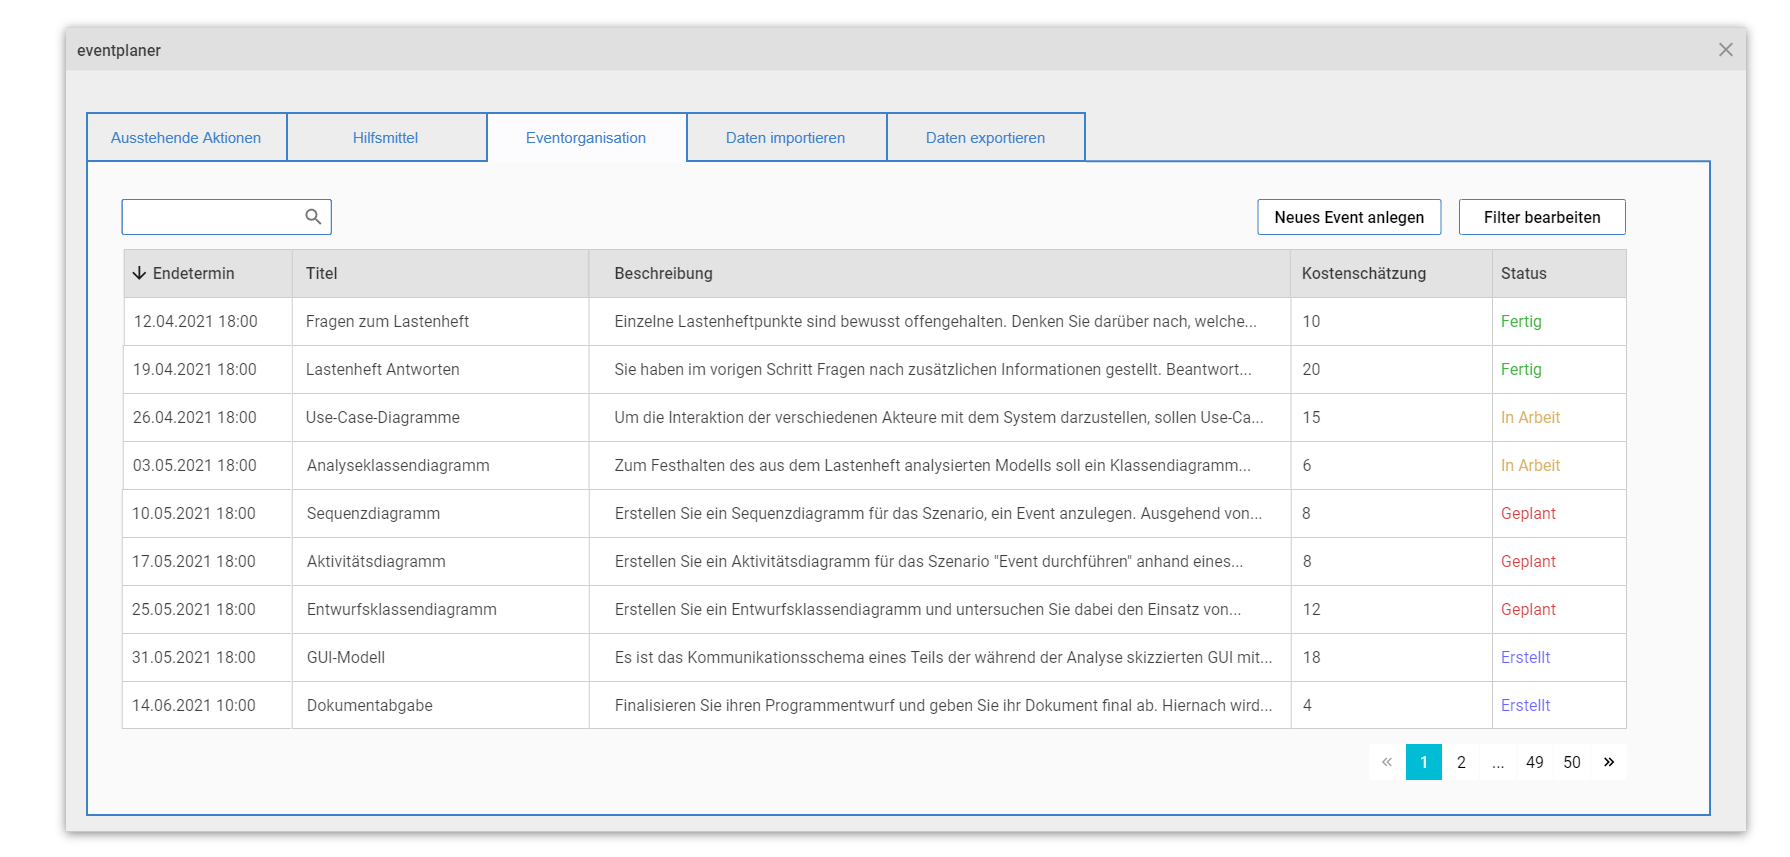
\includegraphics[width=0.98\columnwidth]{Bilder/mockup_eventorganisation.png}
    \caption{Übersicht der Events}
    \label{gui:übersicht-events}
\end{figure}
\newpage
\FloatBarrier
\subsection{Template auswählen}
Möchte ein Organisator ein neues Event anlegen, so hat er die Möglichkeit, dieses auf Basis eines Eventelements, also eines Templates, zu tun. Darum wird ihm beim Anlegen eines Events zunächst das in \autoref{gui:template-auswählen} modellierte GUI angezeigt, sodass er entweder eines der vorgefertigten Templates auswählen oder, falls er mit einem leeren Event starten möchte, \enquote{Blank} auswählen kann.

\begin{figure}[ht!]
    \centering
    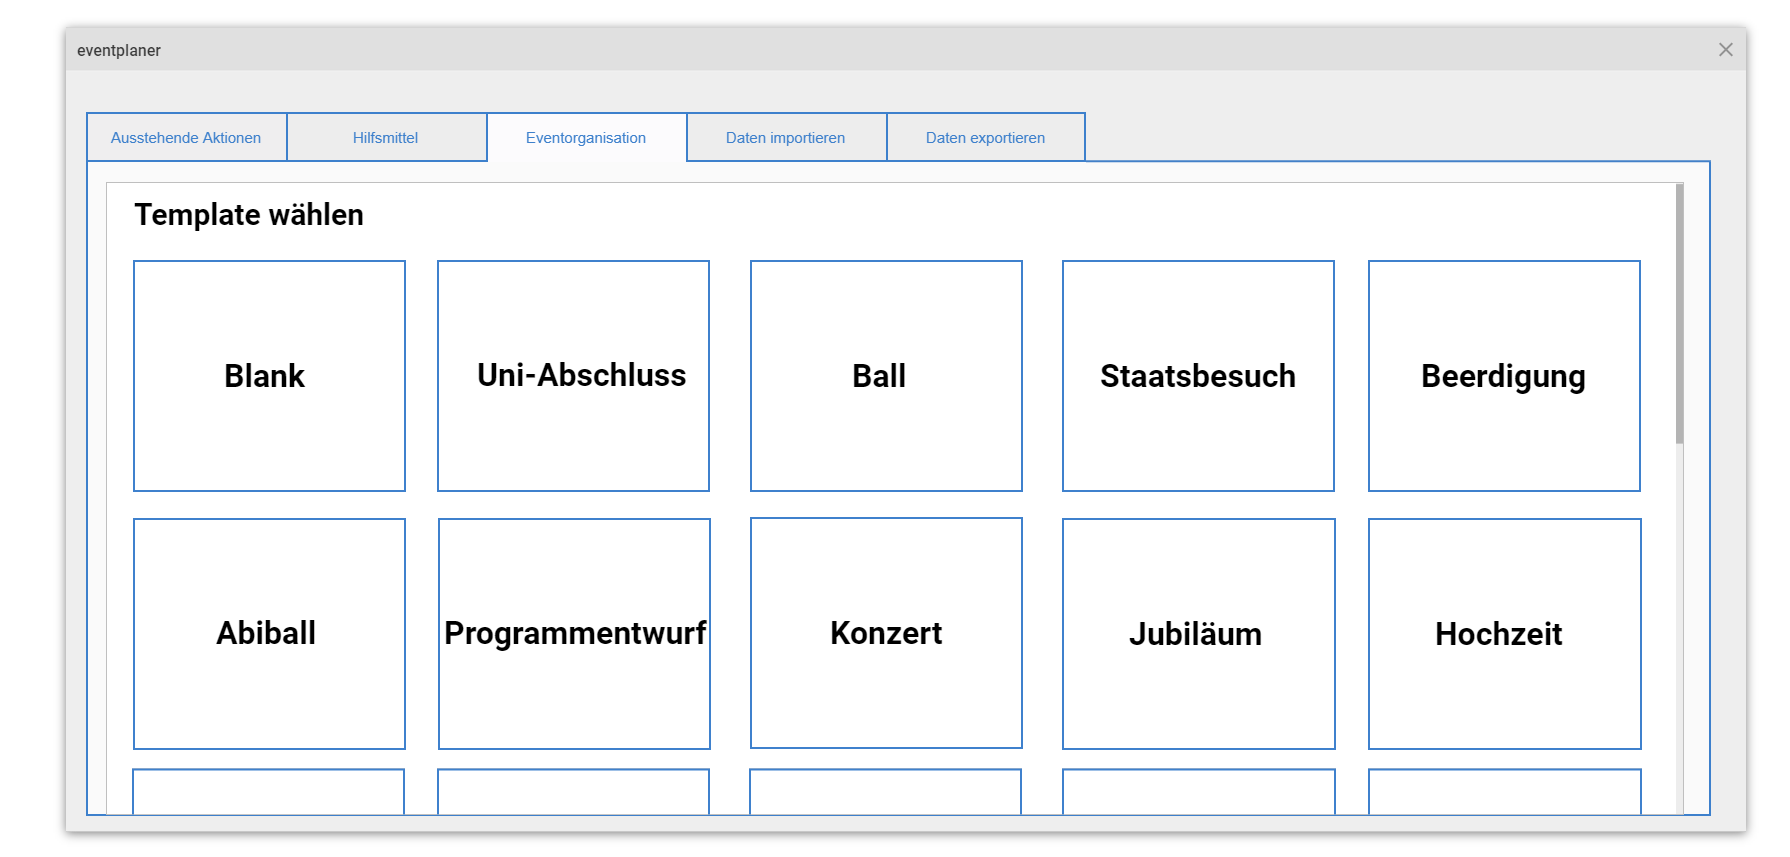
\includegraphics[width=0.98\columnwidth]{Bilder/mockup_neues_event_anlegen_templateauswahl.png}
    \caption{Template auswählen}
    \label{gui:template-auswählen}
\end{figure}

\newpage
\subsection{Neues Event anlegen und Attribute setzen}
Hat sich der Organisator für ein Template bzw. das leere Event entschieden, wird ihm der in \autoref{gui:event-anlegen} gezeigte Screen angezeigt. Hier kann der Organisator die primitiven Attribute Titel, Beschreibung und Kategorie des Events setzen, außerdem werden Start- und Endetermin sowie der Verantwortliche für das Event ausgewählt. Auf der rechten Seite hat der Organisator die Möglichkeit, dem Event in verschiedenen Tabs Verweise, Bilder und untergeordnete Teileinheiten hinzuzufügen.

\begin{figure}[ht!]
    \centering
    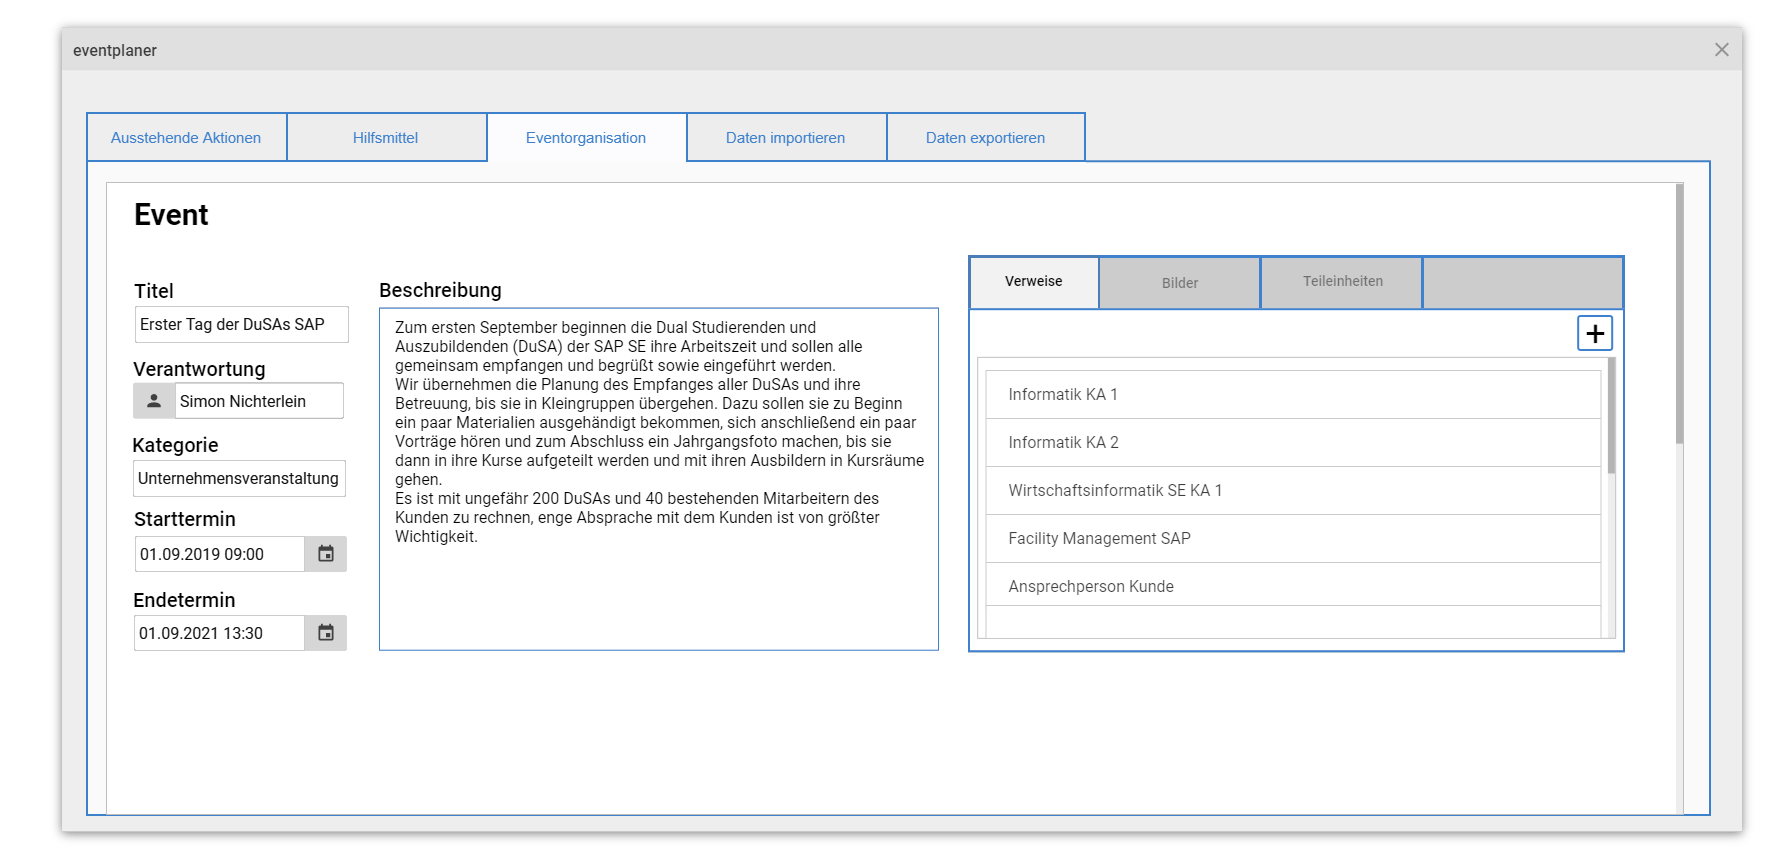
\includegraphics[width=0.98\columnwidth]{Bilder/mockup_neues_event_anlegen_attribute_setzen.png}
    \caption{Neues Event anlegen}
    \label{gui:event-anlegen}
\end{figure}

\newpage
\FloatBarrier
\subsection{Ausstehende Aktionen eines Mitarbeiters}
In der in \autoref{gui:ausstehende-teilevents} gezeigten Ansicht werden jedem Mitarbeiter individuell die ihm zugeordneten Aktionen angezeigt, welche noch nicht abgeschlossen wurden. Um ein einheitliches Look and Feel zu erreichen, werden auch die Aktionen tabellarisch mit den Attributen Endetermin, Titel, Beschreibung, Kostenschätzung und Status angezeigt. Diese können wie die Events im vorherigen Abschnitt ebenfalls gefiltert und durchsucht werden. Auch hier werden diese seitenweise geladen, außerdem sind die Events nach Endetermin sortiert, sodass diejenigen Event ganz oben stehen, welche als nächstes abgeschlossen werden müssen.

\begin{figure}[ht!]
    \centering
    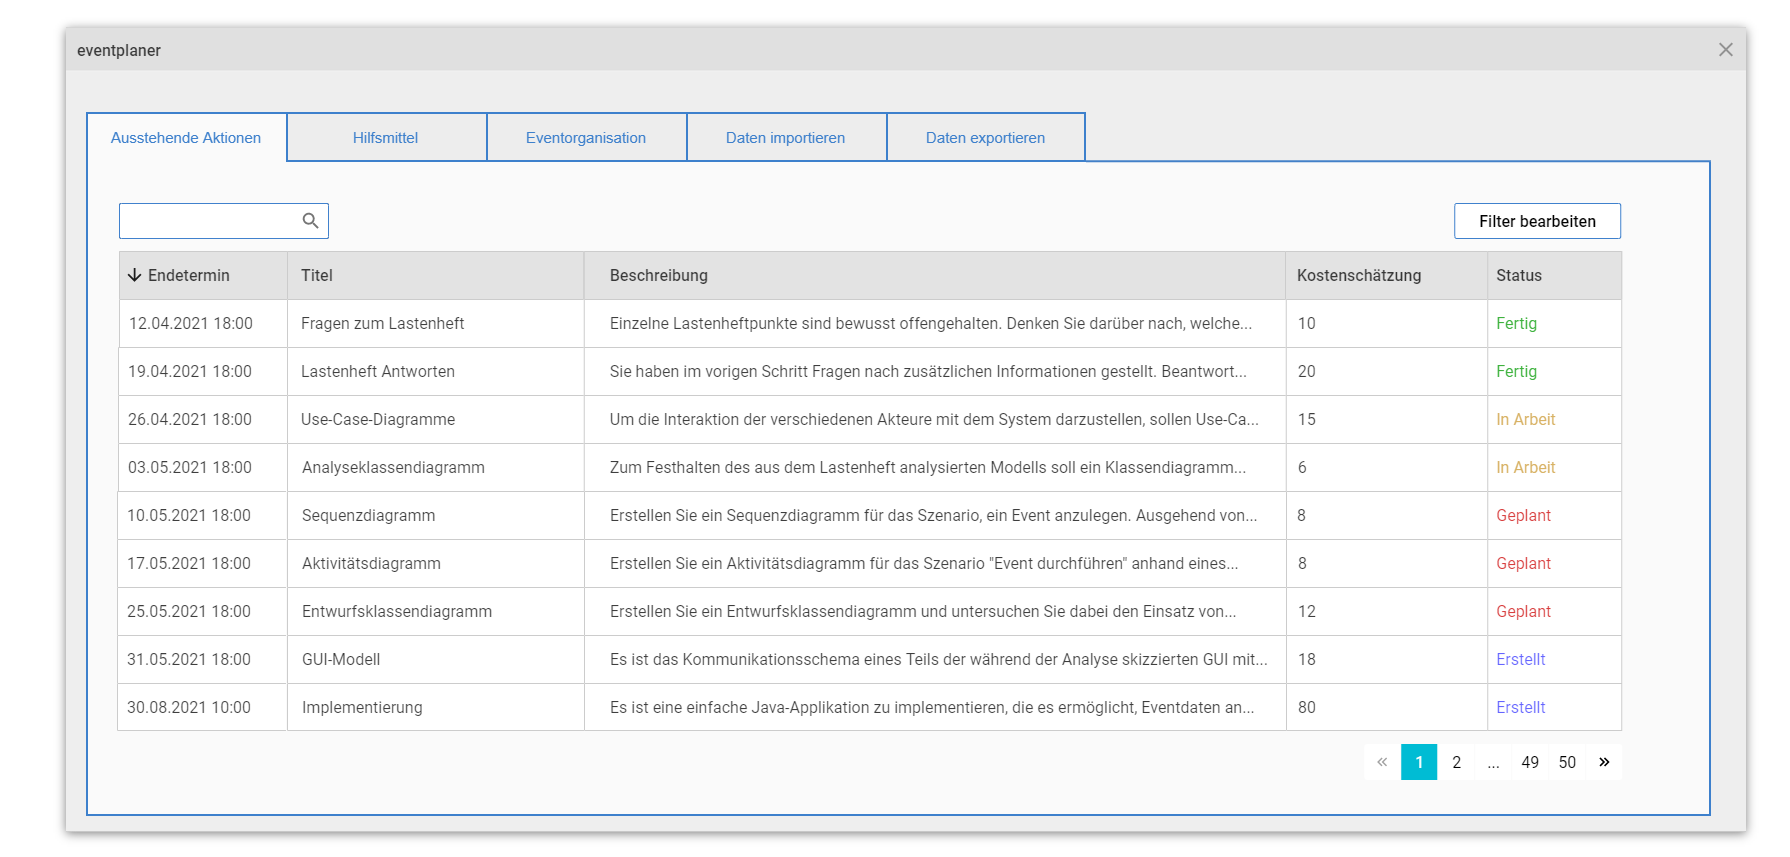
\includegraphics[width=0.98\columnwidth]{Bilder/mockup_ausstehende_teilevents.png}
    \caption{Ausstehende Aktionen eines Mitarbeiters}
    \label{gui:ausstehende-teilevents}
\end{figure}

\newpage
\FloatBarrier
\subsection{Übersicht der Hilfsmittel}
\autoref{gui:übersicht-hilfsmittel} zeigt die Hauptansicht der Hilfsmittelverwaltung, auf der die im System hinterlegten Hilfsmittel tabellarisch angezeigt werden. Zu sehen sind in der Übersicht die Attribute Materialnummer, Name, Lagerort, Menge sowie die Klasse des Hilfsmittels, also ob es sich um ein Gebrauchs- oder Verbrauchsgut handelt. Auch die Hilfsmittel werden seitenweise geladen und können durchsucht und gefiltert werden. Ferner kann mit Hilfe des Buttons \enquote{Gebrauchsgut anlegen} oder \enquote{Verbrauchsgut anlegen} ein neues Hilfsmittel angelegt werden.

\begin{figure}[ht!]
    \centering
    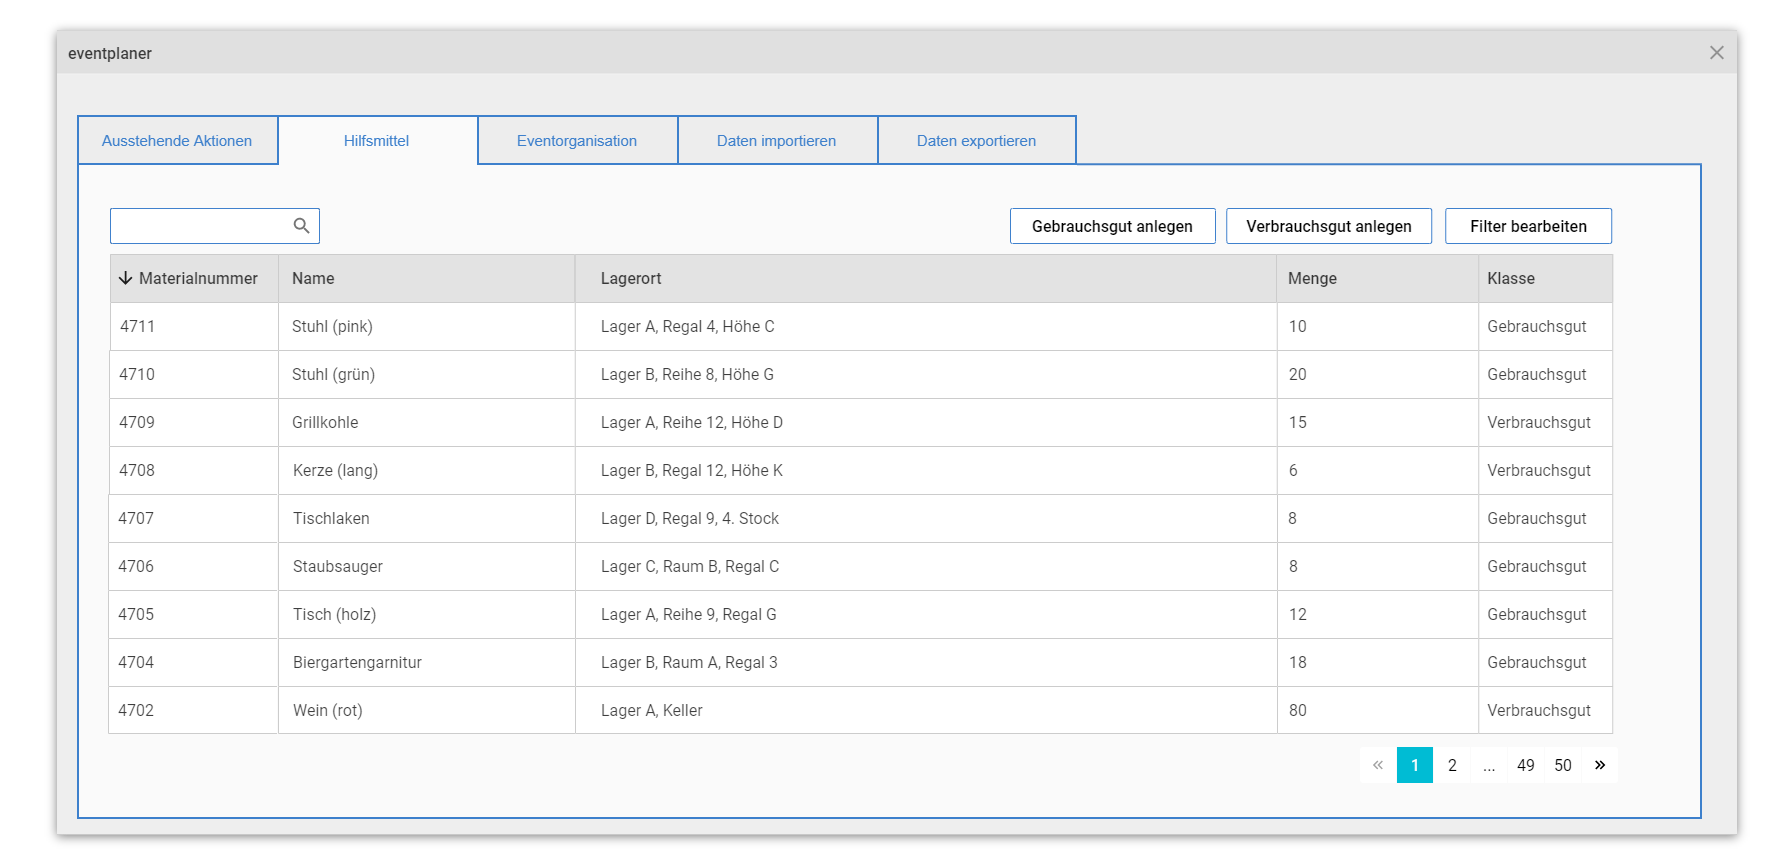
\includegraphics[width=0.98\columnwidth]{Bilder/mockup_hilfsmittel.png}
    \caption{Übersicht der Hilfsmittel}
    \label{gui:übersicht-hilfsmittel}
\end{figure}

\newpage
\FloatBarrier
\subsection{Datenimport}
Das UI für den Import von Events wurde in \autoref{gui:datenimport} modelliert. Hier kann der Nutzer mittels des Buttons \enquote{Datei auswählen} zunächst die CSV-Datei mit den für den Import vorgesehenen Daten auswählen. Diese werden anschließend geladen und in der Tabelle angezeigt, jedoch noch nicht importiert. Als nächstes hat der Nutzer die Möglichkeit, die Events zu filtern. Erfüllt ein Event nicht die Filterkriterien, so wird die entsprechende Checkbox in der Spalte \enquote{Ausgewählt?} ausgegraut und dahinter das Wort \enquote{Filter} angezeigt. Bei den restlichen Events kann der Nutzer mit Hilfe der Checkbox individuell entscheiden, ob er diese importieren möchte oder nicht. Standardmäßig sind alle nicht ausgefilterten Events ausgewählt.

\begin{figure}[ht!]
    \centering
    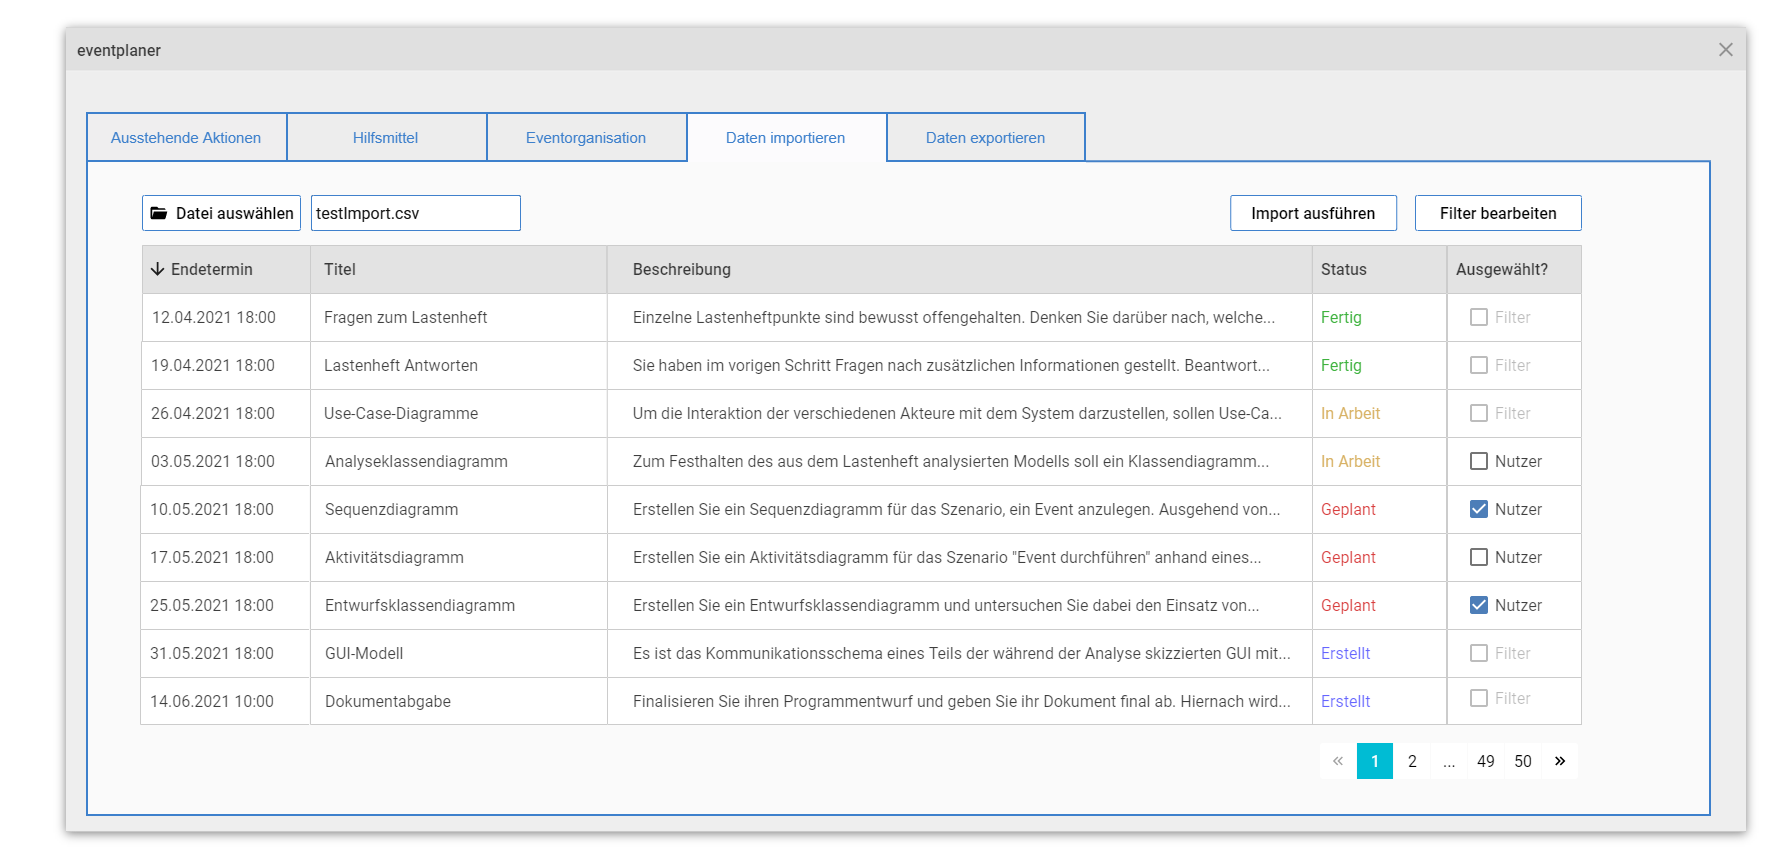
\includegraphics[width=0.98\columnwidth]{Bilder/mockup_daten_importieren.png}
    \caption{Datenimport}
    \label{gui:datenimport}
\end{figure}

\newpage
\FloatBarrier
\subsection{Datenimport mit Filtern}
Klickt der Nutzer während des Imports auf den Button \enquote{Filter bearbeiten}, so ändert sich die Anzeige wie in \autoref{gui:datenimport-filter} gezeigt: Rechts wird weiterhin die Tabelle mit den zu importierenden Events angezeigt, allerdings in kompakterer Form, links können die Filter bearbeitet werden. Dort wird jeder Filter durch eine Zeile repräsentiert. In der linken Zelle steht jeweils das Attribut, nach dem gefiltert werden soll, in der mittleren der logische Vergleichsoperator und ganz rechts der Wert, mit dem verglichen werden soll. Mit dem Button \enquote{Neuer Filter} kann eine weitere Zeile und damit ein weiterer Filter hinzugefügt werden und mit dem Button \enquote{Filter anwenden} wird das Bearbeiten der Filter beendet und diese angewendet.

\begin{figure}[ht!]
    \centering
    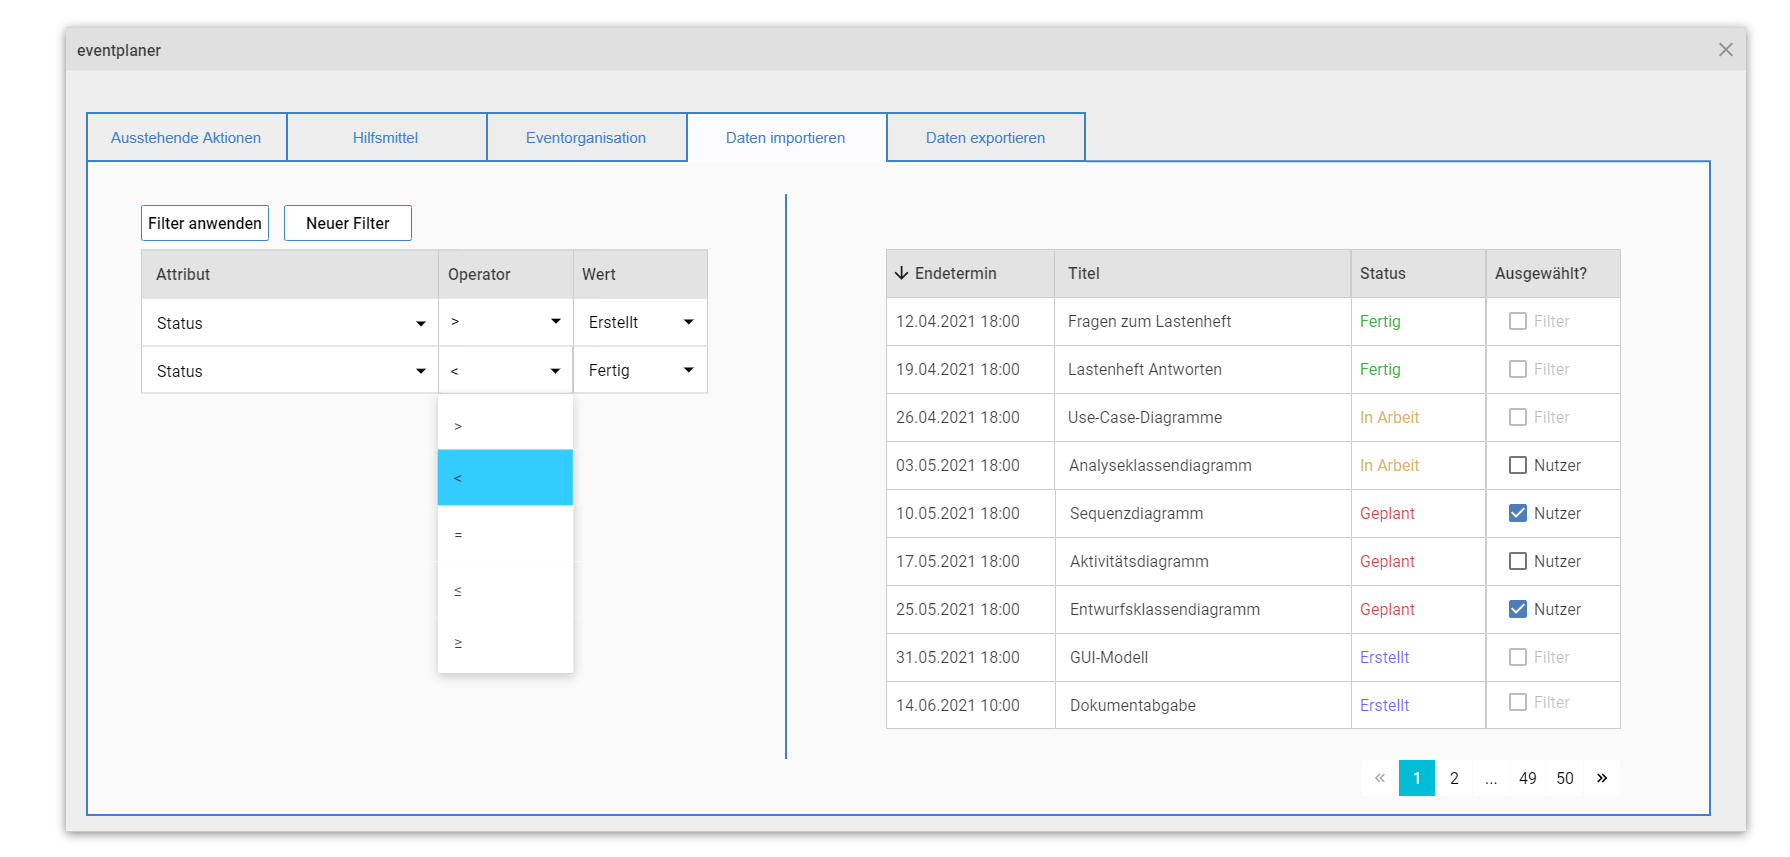
\includegraphics[width=0.98\columnwidth]{Bilder/mockup_daten_importieren_filter.png}
    \caption{Datenimport mit Filtern}
    \label{gui:datenimport-filter}
\end{figure}
